\documentclass[12pt]{article}

\setlength{\textwidth}{6.5in}
\setlength{\textheight}{8.5in}
\setlength{\evensidemargin}{0in}
\setlength{\oddsidemargin}{0in}
\setlength{\topmargin}{0in}

\setlength{\parindent}{0pt}
\setlength{\parskip}{0.1in}

% if you want a double-spaced thesis, uncomment this line:
% \renewcommand{\baselinestretch}{2}

\usepackage{graphicx}
\usepackage{hyperref} % automatically turns citations and the table of contents into PDF links
\usepackage{longtable} % allows for tables that span across more than one page
\usepackage{latexsym}
\usepackage{multirow}
\usepackage{setspace}
\usepackage[table]{xcolor}
\usepackage[nottoc,notlot,notlof]{tocbibind}
\usepackage{pdfpages}
\usepackage[titletoc]{appendix}
\usepackage{tabularx}
\usepackage[ampersand]{easylist}
\usepackage[export]{adjustbox}
\usepackage{wrapfig}
\usepackage{caption}
\usepackage{listings}
\usepackage{tikz}
\usepackage{subcaption} % allows the use of multiple images in a single figure
\usepackage{placeins} % allows the use of the \FloatBarrier command to force images into sections
\usepackage[T1]{fontenc} % allows for certain symbols, such as < and >, to be inserted directly into the text
\usepackage[utf8]{inputenc} % allows for international symbols, like ö, to appear in the text 

\usetikzlibrary{shapes.multipart}
\usetikzlibrary{arrows}
\usetikzlibrary{shapes.geometric}
\usetikzlibrary{positioning}
\usetikzlibrary{trees}

\DeclareFixedFont{\ttb}{T1}{txtt}{bx}{n}{12} % for bold
\DeclareFixedFont{\ttm}{T1}{txtt}{m}{n}{12}  % for normal

% \usepackage{todonotes} % allows for \todo commands

\definecolor{light-gray}{gray}{0.90}
\definecolor{lightgray}{rgb}{.9,.9,.9}
\definecolor{darkgray}{rgb}{.4,.4,.4}
\definecolor{purple}{rgb}{0.65, 0.12, 0.82}
\definecolor{deepblue}{rgb}{0,0,0.5}
\definecolor{deepred}{rgb}{0.6,0,0}
\definecolor{deepgreen}{rgb}{0,0.5,0}

\hypersetup{
    unicode=false,          	% non-Latin characters in AcrobatÕs bookmarks
    pdftoolbar=true,        	% show AcrobatÕs toolbar?
    pdfmenubar=true,        	% show AcrobatÕs menu?
    pdffitwindow=false,     	% window fit to page when opened
    pdfstartview={FitH},    	% fits the width of the page to the window
    pdftitle={Austin Cory Bart's Preliminary Proposal},    	% title
    pdfauthor={Austin Cory bart},     % author
    pdfsubject={Motivating Introductory Computing with Student-Driven Datasets},   % subject of the document
    pdfcreator={Overleaf},   % creator of the document
    colorlinks=true,       % false: boxed links; true: colored links
   linkcolor=black,          % color of internal links
    citecolor=black,        % color of links to bibliography
    filecolor=black,      % color of file links
    urlcolor=black      % color of external links
}

\usetikzlibrary{arrows,positioning} 
\tikzset{
    %Define standard arrow tip
    >=stealth',
    %Define style for boxes
    box/.style={
           rectangle,
           rounded corners,
           draw=black, very thick,
           minimum height=2em,
           text centered},
    % Define arrow style
    arrow/.style={
           <->,
           thick,
           %shorten <=2pt,
           %shorten >=2pt,
					}
}

\begin{document}

\pagenumbering{gobble}

\title{Motivating Introductory Computing with Student-Driven Datasets} 
\author{Austin Cory Bart}
\maketitle     

\newpage
\tableofcontents
\pagebreak
\listoffigures

\newpage   
\section{Summary}

My research is focused on motivating and scaffolding introductory computing experiences.
Non-traditional computing students in courses such as Computational Thinking pose a unique challenge because of their limited motivation and skill, and the scale of such classes.
To overcome these limitations, I propose a novel block-based programming environment leveraging mutual language translation to authentically transition students from the block-based code to a text-based programming language.
The system will use sophisticated program analysis to guide students to success and report learner progress to instructors.
The tool will synergize with a large collection of beginner-friendly big data sources in order to authentically contextualize the learning experience and thereby improve learner motivation.
Data will be gathered on students' motivation and learning progress and instructors' perceptions of the success of the tool in order to answer my hypotheses about the efficacy of the this approach and the tools that are developed to support it.
    
\newpage
\pagenumbering{arabic}
\pagestyle{myheadings}
\setcounter{page}{1}


\pagebreak

\section{Problem Statement}

Computational Thinking is increasingly considered a 21st century competency, paralleling its growing entrenchment within universities’ general education curriculum~\cite{wing2006}.
Although the term itself is historically ill-defined, most definitions consider it the application of computer science concepts and computational techniques to frame problems and devise solutions across disciplines~\cite{weinberg2013}. 
Although Computational Thinking is more than just programming, programming is a key element of Computational Thinking -- and introducing programming is an on-going struggle within the field of Computer Science education.
This struggle is magnified when brought before a more general public, the primary goal of the Computational Thinking movement.

At Virginia Tech, the core requirements at the university have recently shifted to require all undergraduate students to take credit hours in Computational Thinking.
These students represent a diverse spread of majors from the arts, the sciences, engineering, agriculture, and more.
Non-major learners represent a challenge because they have no prior background in computer science, have no assurances that it will be a useful experience, and are not confident about their ability to succeed in the course.
Further complicating these problems is that enrollment for such courses must scale aggressively due to their critical role within new general education requirements -- few departments have the expertise and resources necessary to effectively teach the subject.
At the same time, an active, collaborative learning experience is optimal for meaningfully imparting the course material – lecture should be minimal, and class time should be a chance to work with the material, interact with classmates, and receive support from the course staff.
This primary problem is therefore composed of three pedagogical research questions:
\begin{enumerate}
	\item How do we motivate these unique learners?
	\item How do we guide these learners to achieve success?
	\item How do we scale the instructional materials to as large a population as possible?
\end{enumerate}

This work will develop new pedagogical approaches and technical tools to better understand and resolve these questions.
In particular, we will explore the efficacy of Big Data Science as an introductory context and efficacy of a scaffolded Block-based Programming Environment that utilizes advanced techniques in program analysis and software engineering to guide the learner.


\section{Literature Review}

\subsection{Educational Theory}

There are many elements of the learning process, and many theories of how people learn, how to teach, and how to engage with students. 
In this proposal, I investigate Academic Motivation - the process by which people choose to direct energy towards learning.
Motivation is well understood to be a crucial part of education, particularly in Computer Science~\cite{Carter:2011}.
I apply motivational models against a learning model inspired by Situated Learning Theory in order to focus on the different aspects.

\subsubsection{MUSIC Model of Academic Motivation}

My work uses the MUSIC Model of Academic Motivation as its primary motivational framework.
Although there are many motivational models available, few strive to be holistic models specifically developed for education.
For example, theories like Expectancy-Value and Cognitive Evaluation Theory have a wider scope and have stemmed from other disciplines such as healthcare. %TODO: Cite
The MUSIC Model is derived from a meta-analysis of these other theories, incorporating only the academically relevant components.
Further, the MUSIC model is a tool meant for both design and evaluation, allowing it to be used in all phases of this work.
Finally, the model and its associated instrument, the MUSIC Model of Academic Motivation Inventory (MMAMI) , has been extensively validated and used in other educational domains, making it a reliable device\cite{jones-validity}.

The MUSIC model identifies five key constructs in motivating students \cite{jones-description}.
\begin{description}
	\item[eMpowerment:] The amount of control that a student feels that they have over their learning (e.g., course assignments, lecture topics, etc.). This is amount of Agency that a student perceives.
	\item[Usefulness:] The expectation of the student that the material they are learning will be valuable to their short- and long- term goals. There is no clear delineation of the time-scale for these goals, but there is nonetheless a distinction between strategic skills that students need to be successful in careers and personal interests and the tactical skills they need to complete present-day tasks.
	\item[Success:] The student's belief in their own ability to complete assignments, projects, and other elements of a course with the investment of a reasonable, fulfilling amount of work. Most students desire experiences that are successful, but still challenging enough to be worth it.
	\item[Interest:] The student's perception of how the assignment appeals to situational or long-term, individual interests. The former covers the aspects of a course related to attention, while the latter covers topics related to the fully-identified areas of focuses of the student. It can be difficult to parse out the difference between individual interests and long-term career goals -- there can be alignment between these two components.
	\item[Caring:] The students perception of other stakeholders' attitudes toward them. These stakeholders primarily include their instructor and classmates, but also can be extended to consider other members of their learning experience (e.g., administration, external experts, etc.). It can also be viewed as the extension towards society as a whole.
\end{description}

Students are motivated when one or more of these constructs is sufficiently activated.
They are not all required to achieve maximal levels, and in fact that is not always desired -- it is possible, for instance, for a student to feel too empowered, and become overwhelmed by possibilities.
For some of these constructs, a careful balance is required, and it may not be possible to ever achieve a minimal level; no matter how exciting you make your lecture, you may never convince your students it is interesting, although it is possible that they will still consider it useful and stay motivated.
Crucially, students' subjective \textit{perception} of these constructs is a defining requirement and is more important than objective reality.
It does not matter if you believe that your lecture is Useful, if you have not convinced your students that it is (although an instructor's beliefs are a powerful tool for convincing their students).

The MUSIC model is often used as an organizational framework and an evaluative tool.
As the former, it is a list of factors to consider when building modules, assignments, and content of a course.
At all times, instructors can consider whether they are leveraging at least one construct to motivate their students.
As the latter, it offers both a quantified instrument (MMAMI) and a structure to anchor a qualitative investigation on.
The model has also been used in course design: Jones describes a controlled classroom experiment to motivate students by having an experimental group reflect on how a course satisfies the constructs of the MUSIC model. Students were simply prompted to answer the question ``How will the material presented here be useful to you?''.
Quantitative data gathered after the experiment indicated a significant increase in motivation~\cite{mcginley2014brief}.
The MUSIC model is therefore a flexible resource for studying motivation.

The MUSIC model has not been applied to Computer Science education before, although a number of other motivational frameworks have been leveraged in studies.
Many of these studies often find results that hint at many of the elements of the MUSIC model.
For instance, Mitchell describes interest, usefulness, and ``intellectual challenges'' (success) as three primary elements influencing success in computer science~\cite{Mitchell:2000} .
Although they do not discuss empowerment and social elements, many other studies often suggest these themes.
Still, it should be acknowledged that it is an open question whether the MUSIC model can be applied directly, or if the domain has different characteristics from other disciplines.

\subsubsection{Situated Learning Theory}

A learning experience is a complex sequence of contextualized events, and Situated Learning Theory can help explain the structure of this experience --- and in turn, this structure can be cast against the MUSIC model to explain the motivation over the course of a learning experience.
Situated Learning Theory, originally proposed by Lave and Wenger, argues that learning normally occurs as a function of the activity, context, and culture in which it is situated~\cite{lave-situated}.
Therefore, tasks in the learning environment should parallel real-world tasks, in order to maximize the \textit{authenticity}.
Contextualization is key in these settings, as opposed to decontextualized (or ``inert'') settings.
The key difference is that learning is driven by the problem being solved, rather than the tools available. Therefore, the problem being solved should lead directly to the tool being taught.
This argument suggests that this is a key aspect of motivating students.

Authenticity is a crucial, recurring theme within Situated Learning Theory.
All instruction and assessment must be aligned with reality such that success in the former leads to success in the latter.
However, there is a subtle nuance here -- authenticity is a perceived trait, not an objective one.
Students derive value from their learning only if they \textit{perceive} authenticity, regardless of whether the instructor has successfully authenticated the experience.

Situated Learning Theory has been applied to Computer Science before, with mixed results. A seminal paper by Ben-Ari \cite{ben2004situated} explores its application and limitations.
This paper is somewhat hasty in its application of SL Theory by taking a macro-level view -- they narrowly look to Open-Source and Industry Software Development communities as the only potential Community of Practice and interpret SL Theory as strictly requiring constant legitimacy, largely ignoring the possibility for gradual development of authenticity within individual courses and modules throughout a curriculum:

\begin{quote}
What I am claiming is that situated learning as presented in their work cannot be accepted at face value, because it simply ignores the enormous gap between the world of education and the world of high-tech CoPs, which demand extensive knowledge of both CS subjects and applications areas.
This gap can only be bridged by classical decontextualized teaching in high schools, colleges and universities.
\end{quote}

However, other researchers have found it a useful lens for analyzing curricula.
For instance, Guzdial and Tew \cite{guzdial2006imagineering} used the theory to explore and deal with the problem of inauthenticity within their Media Computation project.
SL Theory clearly has value, but only as a function of the way that it is applied.
In this preliminary proposal, I use SL Theory as a generalized tool for exploring the topic of authenticity throughout introductory Computer Science.

The original work in Situated Learning Theory was not about pedagogy or instructional design. It described how people learn and the importance of context and collaboration, but it did not recommend a particular teaching style.
Subsequent research by Brown \cite{brown1989situated} and others expanded the theory so that it could be applied to the design of learning experiences.
These expansions often naturally dictate the use of active learning techniques, reducing the role of lecture in favor of collaborative, problem-based learning activities.
Choi \& Hannafin \cite{situated-cognition} describe a particularly useful, concrete framework for designing situated learning environments and experiences.
The Choi \& Hannafin framework has four key principles: the Context, described as the ``... The problem's physical and conceptual structure as well as the purpose of activity and the social milieu in which it is embedded''\cite{rogoff1984everyday}; the Content, the information intending to be conveyed to the students; Facilitations, the modifications to the learning experience that support and accelerate learning (commonly done through Scaffolds); and Assessment, the methods used to evaluate the learning experience and measure the progress of the student.
In my research, I focus on the value of the context and faciliations towards motivation, as opposed to the content and assessment.
	
\subsubsection{Contexts vs. Content}

\begin{wrapfigure}{R}{0.5\textwidth}
	\begin{center}
    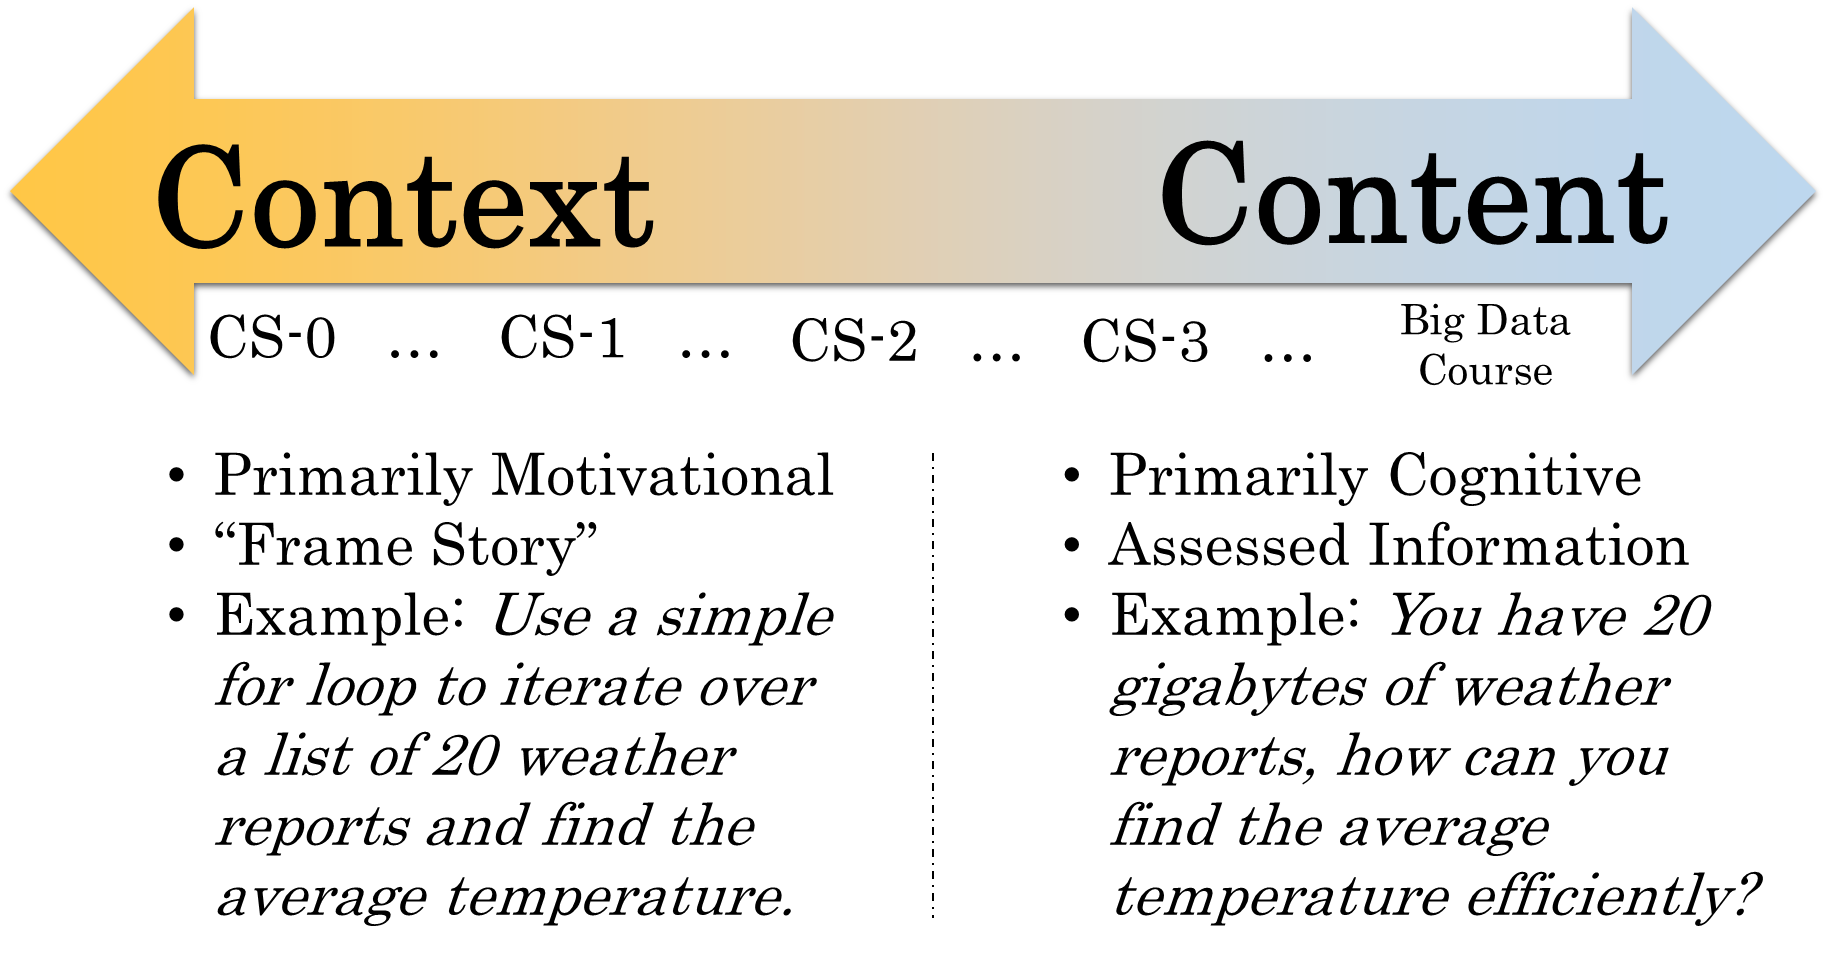
\includegraphics[width=\linewidth]{images/content-context-2.png}
	\end{center}
	\caption{Content vs. Context}
	\label{fig-content-context}
\end{wrapfigure}

There is a reciprocal relationship between contexts and content.
Figure \ref{fig-content-context} demonstrates an example of this relationship for the expected emphasis on big data as a context vs. content throughout an undergraduate curriculum, from a CS-0 (non-majors) course all the way to an upper-level course specifically on big data.
Consider teaching Big Data as a topic: upper-level course could naturally have big data as a context and content, an introductory course would be unlikely to have it as content although it could be used as a framing story for assignments.
Of course, many topics often bring some associated content with it.
When students learn programming in the context of, say, game development, they are almost necessarily learning content related to game development that may not be universal to computer science (e.g., how graphical resources are organized and accessed within the game engine).
This content may be seen as a distraction by the instructor, or as useful side knowledge. For example, if a student had to learn how to use a command line in order to compile their game, they would be learning an authentic skill that might not be considered part of the core content, but is nonetheless generally useful.
When evaluating a context, it is useful to consider what content it represents, and how authentic and useful it is.
The authenticity of content that is attached to a context affects the authenticity of the learning environment as a whole.
A good context enables a student to find recognizable elements and build on prior understanding, eventually being able to freely transfer their learning to new contexts.

Fascinatingly, the need for a strong context diminishes as learners mature and become domain-identified -- the content itself becomes the context.
Learners start to see other contexts as nothing more than distractions and unnecessary fluff.
This makes sense -- you would hope that Computer Science majors in their third semester would be naturally interested in the material, and this is borne out in experimental data.
For instance, Yarosh \& Guzdial attempted to integrate Media Computation in a CS-2 (Data Structures) course, and found that the learners had ``outgrown the desire for a context''~\cite{yarosh2008narrating}. 
These results are similar to results we found in our interventions with a CS-3 couse on Data Structures and Algorithms, where students seemed more irked by the surrounding context than intrigued.


\begin{figure}[!ht]
	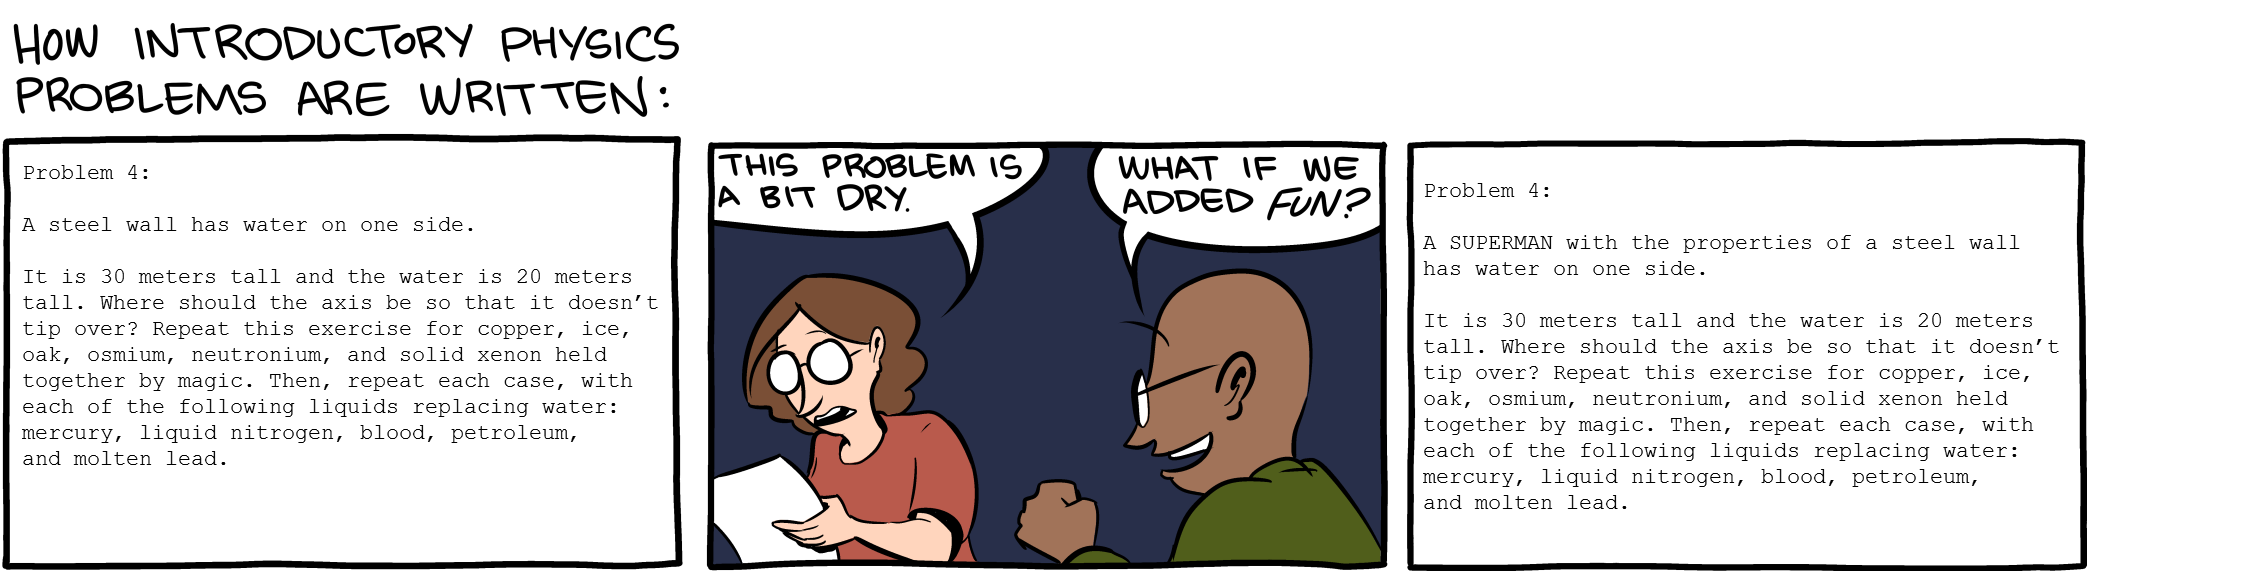
\includegraphics[width=1.1\linewidth]{images/smbc-horizontal.png}
	\caption{How to Add Fun to Education}
	\textit{Making the context ``Fun'' is not necessarily trivial, whether in physics education or computer science education.~\cite{SMBC}}
	\label{fig-comic-context}
\end{figure}

Of course, it is up to the instructor to choose the depth and breadth of the context's integration.
The trade-off between the value and distraction added by the context is a delicate formula.
Consider the scenario in Figure \ref{fig-comic-context}.
A steel wall is a relatively relatable concept for most students -- they can readily imagine such a large, durable object, and it somewhat reasonable to expect that objects would interfere with it.
In this scenario, the instructors consider replacing the wall with a comic book character -- something that they anticipate will be more ``fun''.
If they are in tune with their learners, this might be an effective context -- perhaps they know that their learners are comic book fans.
However, because the integration is only at the surface level, it is possible that the learners will see this as a forced reference, and they will have a more negative reaction.
It is also possible that they will not recognize the reference, or feel no positive emotions with it -- many contexts do not take into account gender, racial, or socio-economic characteristics of the anticipated learner.
I suggest that the process of motivating students using a context is non-trivial, and in the following section I will explore prior work in contexts for Computer Science Education.

\subsection{Introductory Computing Content}

Different Computer Science programs have different introductory curriculums, varying on whether they focus on Object-Oriented programming, Functional programming, etc. 
Complicating this discussion is the bifurcation of undergraduate introductory computing into Computational Thinking (sometimes referred to as CS-0) and Computer Science (sometimes referred to as CS-1), and the simplified curriculums used in K-12 education (e.g., the new AP CS course).
However, It is commonly that any good introductory computing course will cover abstraction (representing complex phenomena more simply, usually as coded data), some form of decision-making (e.g., \texttt{if} statements, \texttt{cond} statements), and some form of iteration (e.g., \texttt{for} loops, recursion)~\cite{Kramer:2007, CS2013, csta-computational-thinking}.
From there, different curriculums lay out the material differently.
The ``How to Design Programs'' curriculum emphasizes a functional programming model, using a LISP-descended language named Racket, and the only looping mechanism that students are taught is recursion.
The dominance of the Object-Oriented Model in software engineering usually leads to a strong emphasis in introductory courses on abstracting data using Objects and Classes -- such as the ``Objects First'' curriculum.
Besides the technical aspects, definitions include softer skills such as a tolerance for unstructured problems and collaborative attitudes~\cite{csta-computational-thinking, google-computational-thinking}.

This proposal does not take a view on what should be included in an introductory experience, beyond a core of Abstraction and Algorithms.
However, for practical purposes, materials and research work are grounded and tested in some course, and have adaptions for that content.
Specifically, the proposed work is used in a Computational Thinking course, so that is how the content is oriented.
``Computational Thinking'' was coined by Seymour Papert in 1993~\cite{papert1996} and popularized by Dr. Jeannette Wing's 2006 paper~\cite{wing2006}, which opened a floodgate of discussion about the term. 
Unfortunately, there is still limited consensus on \textit{what} exactly CT is, whether it should be universally taught, how it should be taught, and how to identify when it has been taught.

An excellent resource for summarizing the history of Computational Thinking research is the 2013 dissertation by Wienberg~\cite{weinberg2013}. 
This comprehensive survey analyzed 6906 papers directly or indirectly related to Computational Thinking from 2006-2011, describing research efforts and findings.     
Over half of the research on CT describes approaches to pedagogy (Curriculum and Program Description), leaving a small amount to modeling (Philosophy and Opinion) and assessment (Research and Evaluation). 
The lack of assessment research is understandable given the youth of this area of research, but still troubling.
Even more troubling, however, is the further analysis of the 57 empirical studies.
Only fifteen (26\%) studies include or sought an operational definition of computational thinking, and only six go beyond the superficial (solely describing computational thinking as a ``way of thinking'', a ``fundamental skill'', or a ``way of solving problems''). 
The failure to identify an operational definition weakens the theoretical strength of the studies.
This weakness likely stems from the background of the researchers: only 18\% of the articles involved education experts.
In other words, over four-fifths of this educationally-oriented research appears to have been performed by people with no real formal training in educational research techniques.
This is particularly troubling given that Computational Thinking is a strong target for interdisciplinary endevaors.

Weinberg reflects on the continuing debate about the importance of Computational Thinking:
\begin{quote}
    Many, like Wing, believe computational thinking to be a revolutionary concept, one as 
important to a solid educational foundation as are reading, writing, and arithmetic (Bundy, 2007\cite{bundy2007}) 
(Day, 2011\cite{day2011}). Others believe its potential and significance are overstated (Denning, 2009\cite{denning2009}; 
Hemmendinger, 2010\cite{hemmendinger2010}), and some have voiced concern that by joining forces with other 
disciplines computer science might be diluting either one or both of the participating disciplines 
(Cassel, 2011\cite{cassel2011}; Jacobs, 2009\cite{jacobs2009}). Both the praise and the criticism for computational thinking could 
perhaps be tempered by reflecting on a historical quote by Pfeiffer in 1962: “Computers are too 
important to overrate or underrate. There is no real point in sensationalizing or exaggerating 
activities which are striking enough without embellishment. There is no point in belittling 
either.” (Pfeiffer, 1962\cite{pfeiffer1962}).
\end{quote}

Although it is ambiguous what Computational Thinking is, we will take it as a given that it requires students to learn some amount of non-trivial programming: using iteration constructs (e.g., \texttt{while}, \texttt{for each}, recursion, etc.), decision constructs (e.g,. \texttt{if}, \texttt{unless}), have some sense of program state (through mutating variables or passed through composed functions), and require the programmer to translate instructions into a form the computer can understand.
This is not meant to be a strict definition of everything a programmer should learn -- simply an acceptable, minimal subset.

\subsection{Introductory Computing Contexts}

As part of the overarching goal to bring more students into Computer Science, a large number of contexts have been explored in Introductory computing. 
The context of a learning experience grounds the learner in what they already known, in order to teach the new material.
Many introductory computing experiences focused on presenting the content as purely as possible, which can come across as abstract and detached~\cite{Zografski}.
However, starting with Seymour Papert's work with robotics and the LOGO programming environment in the 70s~\cite{papert1996}, instructors have been interested in motivating students' first experience with richer contexts.
Some of these contexts rely on Situational Interest (e.g.,  Digital Media ``Computation'' (Manipulation)~\cite{Forte} and Game Design~\cite{Zografski}), while others attempt to provide enduring career value (e.g., [Big] Data Science ~\cite{Anderson}) or short-term social applicability (e.g,. Problem Solving for Social Good~\cite{SocialGoodinComputingEducation}).
Ultimately, each of these approaches draws on different facets of motivation, they may be compatible with each other.
In this section, I will discuss the implications of these different approaches.


\subsubsection{Abstract Contexts}

Denning describes the early perception of Computer Science by the public as ``stodgy and nerdy''~\cite{Denning:2005}, since many early computer science classes were driven so strongly by mathematics and logic.
A common early introductory programming problem, for instance, is writing a function to compute a Fibonacci number -- a relatively simple task if you are familiar with the recurrence, and one that leads quite nicely to discussions on the implementation of algorithms, computational complexity, and a host of other subjects~\cite{crazypantsfibonaccipaper}.
These contexts are ``abstract'' because they are already at a similar level of abstraction as the content they are attempting to convey.
However, Oliveira~\cite{ConcreteVsAbstract} suggests that the discussion about ``abstract vs. concrete'' contexts is a misleading one, because the purity with relation to the content is less important than \textit{prior knowledge}.
According to modern constructivist and cognitivist theories, learners build on prior knowledge, and the ability to relate to what they know is crucial.
The simple fact is that most students are not particularly good at mathematics, so relying on it as a context is not a useful approach compared to finding subjects that students know and understand readily.

\subsubsection{Situationally Interesting Contexts}

As it became clear that Computer Science had a serious image problem, work began on making Computer Science ``fun'' and approachable. 
A key goal was to increase diversity and to broaden participation. 
This led to the rise of Situationally Interesting Contexts, emphasizing problems and projects that would be immediately appealing to a wide audience.
Guzdial, for instance, was largely responsible for the creation of the Media Computation approach, where students use computational techniques (e.g., iteration and decision) to manipulate sound, images, videos, and other digital artifacts.
As an example, students might use a nested, numerically-indexed \texttt{for} loop in order to adjust the red-value of the pixels in an image, treating it as a two-dimensional array of binary tuples, in order to reduce the red-eye of a photo.

Although wildly deployed, a review of these curricular materials by Guzdial \cite{guzdial2006imagineering} in light of Situated Learning Theory found that students did not find this an authentic context, and intense rhetoric was insufficient to convince them that it was authentic. 
Few students find it expedient and helpful to remove the red-eye from family photos by writing python scripts, and so are unconvinced that the context has long-term value to them (regardless of whether the content does).
Guzdial leaves open the question of what contexts can be truly authentic for non-majors, given the relative novelty of teaching introductory computing for non-majors.
Ben-Ari echos this question by suggesting a very narrow selection of authentic contexts and communities in his paper exploring the application of Situated Learning Theory to Computer Science in general \cite{ben2004situated}.
Critically, the opposite problem could occur -- if an instructor is effective at convincing students that a context is authentic, the students may believe the instructor even if the context is not authentic.
There are serious ethical issues involved in mispresenting the utility of a context, leading students to develop an embarrassing misconception of the field. Imagine a young child believing that all of Computer Science is game design, because that is what they started off doing.

There are other disadvantages of an Interest-driven approach.
The motivation literature describes ``Seductive Details'' (interesting but irrelevant adjuncts)~\cite{harp1998seductive} as interfering both with short-term problem completion and long-term transfer.
In other words, students get hung up on unimportant aspects of the context, so that they ignore the content.
Consider a student using the game and animation development environment Scratch, which allows beginners to create sprites from images.
A young learner might be so amused by the ability to change the color and shape of their image, that they neglect their assigned work.
Although a well-regulated learner would not be distracted, most of the at-risk population that would benefit from these contexts are unable to deal with such distractions.
Of course, this could be said of any context, but there is particular danger from a seductive context.

Kay~\cite{Kay:2011} identifies another, potentially critical problem of relying solely on situationally interesting contexts, particularly when it leads to individualized interest towards that context and not the content. 
What happens once a student has completed the introductory course and is ready to move onto further courses?
Most later courses are more decontextualized, and will not use contexts such as game development, robots, etc.
Kay goes so far to say that it is unethical to suggest to students that a contextualized introductory course is representative of the curriculum as a whole.

\subsubsection{Empowered Contexts}

Orthogonal to the idea of making a context fun is the idea of giving students more freedom and agency to control their learning.
Compared to Interest-driven contexts, this approach is comparatively less researched, although it is not an uncommon practice. Instructors will often allow students to choose from a range of projects or assignments.
Stone~\cite{EmpowermentInProjects} ran a 2-year study where students were allowed to choose their projects from a wide range of domain areas (e.g., Biology, Math, Business, Etymology), and were then surveyed on their engagement.
Unfortunately, their experiment suffered strongly from low enrollments and even lower survey responses. Therefore, it is difficult to believe any of their results (including the idea that women are more likely to prefer biological- and meterological-themed projects).
However, their experiences do suggest an interesting challenge: normalizing the difficulty (both in terms of computational knowledge and domain knowledge) across many different projects is a struggle.

\subsubsection{Contexts that Make Instructors Care}

Most modern educational theories argue that learning is inescapably affected by social factors.
There is evidence that the instructor~\cite{thompson2009engine} and fellow students~\cite{Barker:2009} are the most important factors in an introductory experience, for instance.
Kay~\cite{Kay:2011} discusses this explicitly.
It is possible that the most important element in a context is not whether it is fun or useful, but whether the instructor can get excited about it and impart that enthusiasm to the student.
And not just enthusiasm, but a thorough understanding of the problem, its usefulness, and the rest of its attributes.

\subsubsection{Useful-Driven Contexts}

An alternative focus to Interest is Usefulness, the idea that the context should have immediate or eventual benefit to the learner's needs.
To some extent, it is impossible (or at least prohibitively difficult) to find a one-size-fits-all context that will be useful to all learners (designing learning experiences without your learners in mind is an example of preauthentication~\cite{preauthentication}).
The ideal situation for any instructor is to create contexts that specifically suit the interests and values of your learners~\cite{DiSalvo:2011}.
However, in practice, some contexts are broadly useful and are likely to engage a diverse crowd of learners.
In this section, I suggest two distinct contexts that might fall into this role: real-world problem solving and data science.

In theory, Computer Science provides tools for solving problems, and it is possible that the problem solving can be done with even the simplest tools~\cite{Layman:2007, SocialGoodinComputingEducation}.
An ITiCSE Working Group collaborated to produce a new framework centered around these ideas -- ``Social Computing for Good'', a collection of approaches and projects for interdisciplinary students to solve using computing ~\cite{SocialGoodinComputingEducation}.
They raise a number of issues with using socially relevant materials: that games and graphics can appeal to instructors as a ``cheap'' source of motivation, that students and instructors can become cognitively overloaded by the addition of domain knowledge, and that instructors can even be intimidated if they don't have expertise in the domain area.
The working group also create a valuable rubric for developing and evaluating problems (which I map to elements of the MUSIC model below):
\begin{enumerate}
	\item The degree to which the problem is student-directed (eMpowerment)
	\item The amount of scaffolding needed (Success)
	\item The amount of external domain knowledge needed (Success)
	\item The contribution to the Social Good (Usefulness, Caring)
	\item The ``coolness'' or ``sexiness'' (Interest)
	\item The amount of explicit student reflection incorporated (Usefulness)
\end{enumerate}
Although this framework presents some ideas, there are still unsolved technical and pedagogical problems in how to optimally bring these materials to learners. Their paper ends by raising questions about the effectiveness of this approach compared to existing methods.

A number of other researchers have created course materials along similar lines.
Erkan~\cite{Erkan:2012} had a sustainability themed curriculum -- student surveys suggested some level of effectiveness, although the sample size (N=16) was far too small to generalize the results.
In addition to providing two case studies, Buckley ~\cite{Buckley:2008} suggests an interesting delineation between Social problems (uppercase S, indicating problems general to society) and social problems (lowercase S, indicating problems of personal interest to the learner).

Barker ran a large survey asking why students persist towards majoring in CS~\cite{Barker:2009} (N=113, only freshmen) and performed a factor analysis.
Critically, they found that Meaningful/Relevant Assignments (subsuming both Interest and Social Usefulness) were a major factor in whether students would persist in the major -- however, it wasn't one of the primary factors (that is, students suggested other factors were more important for deciding whether they would persist).
Interestingly, whether students felt that their workload and pace was appropriate was a much bigger source of importance, suggesting that care and attention should be given to making a context suitably difficult before it is made interesting and useful.
This focus on ensuring normalized, appropriate difficulty is echoed by several other authors, all of whom suggest that doing so is not trivial~\cite{Rader:2011, Stevenson:2006}.

In the past two decades, the field of Data Science has emerged at the intersection of Computer Science, Statistics, Mathematics, and a number of other fields.
This field is concerned with answering real-world problems through data abstractions, and offer a less socially-conscious path to Usefulness.
As a context, there are pedagogical penalties for using it, since it introduces a wide variety of new content including visualization, statistics, ethics, and social impacts ~\cite{Anderson:2015-DP2}.
However, a good instructor can downplay the focus on these side-areas as needed, or even emphasize subject matter's strengths (e.g., a statistics major might find it interesting to use their mathematical background to strengthen their problem-solving investigation).
However, there are other difficulties. Bringing in messy data requires real sophistication by the instructor, especially when working with Big Data.

The use of data analysis as a form of contextualization is not novel, and represents a new and actively growing movement where instructors create programming assignments with specific datasets in mind ~\cite{Anderson, Sullivan:2013, Hall-Holt:2015, DePasquale:2006}.
Upper division courses have employed these situated learning experiences using data of varying size and complexity for several years \cite{Egger, datamining, Waldman}.
However, in all of these research papers, there is typically little evaluation of the advantages and disadvantages of using data science in introductory education.
Although Sullivan ~\cite{Sullivan:2013} did conduct a study on the difficulty and usefulness of the datasets they provided, they do not go far in identifying lasting lessons for educators creating such datasets.
Other researchers conducted even less impressive studies: DePasquale~\cite{DePasquale:2006} included exactly ONE student response in their evaluation.

\section{Datasets as a Holistic Motivating Context}

\begin{figure}
    \begin{center}
    	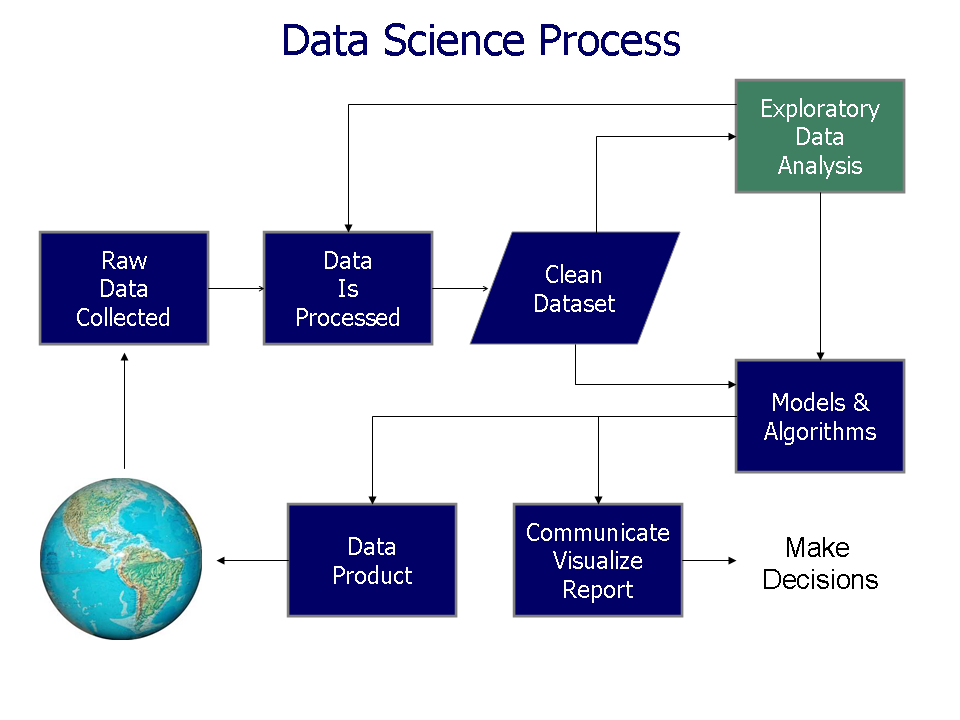
\includegraphics[width=.5\linewidth]{images/data-science.png}
    \end{center}
    \caption{A generalized model of Data Science\protect\cite{data-science-diagram}}
    \label{fig-data-science}
\end{figure}

I propose using datasets as a motivating introductory computing context.
\textbf{My core thesis is that data science, used properly, is an excellent context for motivating students across multiple components of motivation: providing opportunities for agency, a sense of usefulness and authenticity, controllable complexity, the potential to be interesting situationally and towards individualized interest, and a promotion of caring and ethics.}
Data Science accomplishes this by being a ``meta-context'' -- it is a general framework for working with an infinitely wide array of different data contexts.
However, there are many challenges in doing so -- managing data is tricky and can be a very unstructured problem.
For introductory students, in fact, it can be too overwhelming to find and dive into an arbitrary dataset, requiring significant scaffolds to get anywhere.

As established in the previous subsection, this is not a novel approach -- upper forms have always historically used datasets in courses on Machine Learning and Database Design, and recently lower forms have started too~\cite{Anderson}.
However, there is very little evaluation of the success of this approach, and numerous roadblocks exist in using this context.
For my dissertation, I will investigate what technology can be used to take full advantage of this context according to a number of constraints.
Before describing what I have done and will do, however, this section will describe this context in more detail.

\subsection{Data Science}

Data science is the process of answering questions by building, exploring, and processing datasets.
There are many theoretical models that define the term more strictly, but in general it is described as an iterative model of collecting, sanitizing, processing, rendering, and interpreting.
Figure \ref{fig-data-science} gives a visual overview of this process.
My research will not attempt to narrowly define data science; instead, the goal is simply to use elements of the data science process to contextualize the experience of learning about computing topics such as abstraction and algorithms.

It is crucial to understand that the goal is not to teach students how to become data scientists, anymore than it is the goal of Media Computation to teach students how to be professional computational artists.
As a context, using datasets is simply a means to an end -- it may involve any components of the generalized data science process at any level.
Some professors may identify data science as a learning objective in and of itself. That is fine, but they are attempting to teach something that is, at some level, distinct from computing itself.

\subsection{Big Data}

\begin{figure}
    \begin{center}
    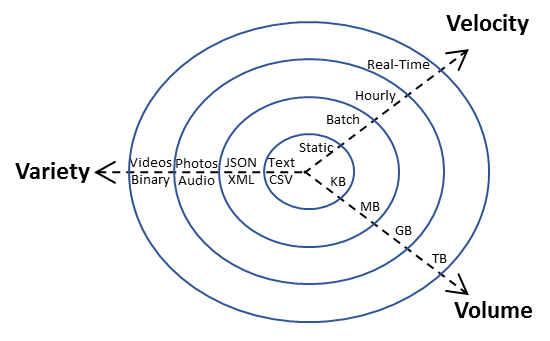
\includegraphics[width=.5\linewidth]{images/3v-model.png}
    \end{center}
    \caption{The 3V Model of Big Data}
    \label{fig-3v}
\end{figure}

One particularly important subtype of datasets is known as Big Data. Big Data is much in the news these days, from reports of massive data
dredging by the NSA to tens of millions of credit cards stolen by
hackers from commercial databases.
Big Data has become crucial to scientific advances from understanding the genome to predicting climate change.
Even more so than regular data science, there are many obstacles to effectively educating students on Big Data.
Its representation, manipulation, and expression is, by definition, challenging, and modern curriculum and programming tools are typically inadequate.

Big data has been loosely described as quantities of information that cannot be handled with traditional methods ~\cite{McKinsey}.
But ``traditional methods'' is a vague phrase that has different meanings to different learners. To a Humanities major in their first CS-0 course, the traditional method to sum a list is to use Excel. In this scenario, ``big data'' means anything that won't comfortably fit into Excel's working memory.
However, to a third-year Computer Science major, the traditional method would be to write an iterative or recursive sequential loop; being given big data forces them to explore parallel models of execution.
Clearly, ``bigness'' is a function of the learner's experience, but that is still not a solid definition.
A more precise definition is the ``3V Model'' \cite{douglas2012importance}, which posits that there are three dimensions that distinguish big data from ordinary, run-of-the-mill data:

\begin{description}
	\item[Volume:] The total quantity of the information, usually measured in bytes or number of records. However, this also extends laterally: the number of fields in the structure of the data also impacts the complexity and size. The threshold at which data becomes big is a function of the hardware and software being used. For instance, embedded systems may consider gigabyte-sized files to be big, while modern servers might not struggle until the petabyte level.
	\item[Velocity:] The rate at which new information is added to the system. High velocity big data implies a distributed architecture, since new data must be arriving from somewhere. The dynamicity of data can vary widely across these architectures, with data updating every year, every day, or even multiple times a second.
	\item[Variety:] The format or formats of the data. Ideally, data are always distributed in a way that is readily accessible. For instance, simple text-based formats such as CSV and JSON are widely supported, relatively lightweight, and human-readable. More sophisticated data formats for image and audio are also typically well-supported, although still more complicated. However, projects using specialized, compressed binary formats or, more dangerously, multiple formats (e.g., image archives organized with XML files), are more complex.
\end{description}

Silva~\cite{Silva:2014} taught an introductory course truly focused on techniques for tackling Big Data: NoSQL, MapReduce, NewSQL.
Unfortunately, they did not conduct any kind of evaluation of their work across any of the expected dimensions. 
Learning to work with Big Data can add extra authenticity to the context, but it also raises a large number of new challenges.
Once again, it is not the goal of my research to teach students how to work with truly Big datasets. Instead, I will explore whether the use of Big Data is a useful means to motivate students.
\section{Big Data Science}

Big Data is much in the news these days, from reports of massive data
dredging by the NSA to tens of millions of credit cards stolen by
hackers from commercial databases.
Big Data has become crucial to scientific advances from understanding the
genome to predicting climate change.
Unfortunately, computer scientists in the workforce are woefully
unequipped for this shifting paradigm.
Indeed, a report by MGI and McKinsey's Business Technology Offices
declares that ``by 2018, the United States alone could face a
shortage of 140,000 to 190,000 people with deep analytical skills as
well as 1.5 million managers and analysts with the know-how to use the
analysis of Big Data to make effective decisions.''\cite{McKinsey}
There are many obstacles to effectively educating students on Big
Data.
Its representation, manipulation, and expression is
challenging, with modern curriculums and programming tools being
inadequate.

\begin{wrapfigure}{r}{0.5\textwidth}
    \begin{center}
		    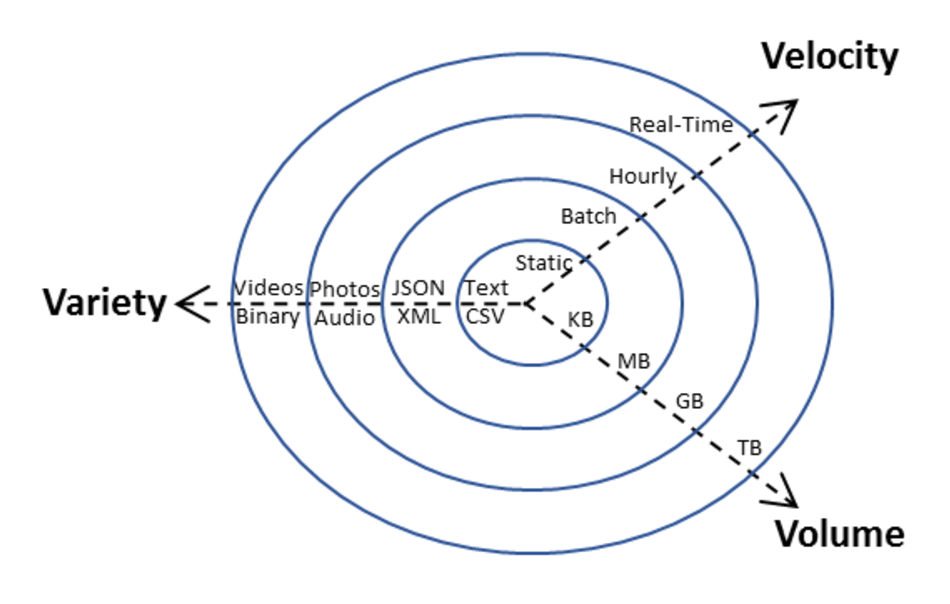
\psfig{file=images/3v-model.eps, width=\linewidth}
    \end{center}
    \vspace{-\bigskipamount}
    \caption{The 3V Model of Big Data}
    \label{fig-3v}
\end{wrapfigure}

Big data has been loosely described as quantities of information that cannot be handled with traditional methods ~\cite{McKinsey}.
But ``traditional methods'' is a vague phrase that has different meanings to different learners. To a Humanities major in their first CS-0 course, the traditional method to sum a list is to use Excel. In this scenario, ``big data'' means anything that won't comfortably fit into Excel's working memory.
However, to a third-year Computer Science major, the traditional method would be to write an iterative or recursive sequential loop; being given big data forces them to explore parallel models of execution.
Clearly, ``bigness'' is a function of the learner's experience, but that is still not a solid definition.

A more precise definition is the ``3V Model'' \cite{douglas2012importance}, which posits that there are three dimensions that distinguish big data from ordinary, run-of-the-mill data:

\begin{description}
	\item[Volume:] The total quantity of the information, usually measured in bytes or number of records. However, this also extends laterally: the number of fields in the structure of the data also impacts the complexity and size. The threshold at which data becomes big is a function of the hardware and software being used -- for instance, embedded systems may consider gigabyte-sized files to be big, while modern servers might not struggle until the petabyte level.
	\item[Velocity:] The rate at which new information is added to the system. High velocity big data implies a distributed architecture, since new data must be arriving from somewhere. The dynamicity of data can vary widely across these architectures, with data updating every year, every day, or even multiple times a second.
	\item[Variety:] The format or formats of the data. Ideally, data are always distributed in a way that is readily accessible -- for instance, simple text-based formats such as CSV and JSON are widely supported, relatively lightweight, and human-readable. More sophisticated data formats for image and audio are also typically well-supported, although still more complicated. However, projects using specialized, compressed binary formats or, more dangerously, multiple formats (e.g., image archives organized with XML files), are more complex.
\end{description}

In the remainder of this section, I describe common challenges associated with different kinds of data.

\subsection{High Velocity Data}

It is not trivial to enable introductory students to work with high velocity data, which is necessarily distributed. Without any scaffolding, it is necessary to delay the use of such data until much later in the course. In a prior paper \cite{realtimeweb-splashe}, we outline the biggest barriers to high velocity data as a context:
\begin{description}
  \item[Access] The process of programmatically downloading and parsing a web-based resource is a non-trivial procedure requiring an understanding of both basic concepts (e.g., function calls, data transformation) and specialized web technology (e.g., the difference between GET and POST calls, building query parameters).
	\item[Non-Idempotency] Because high velocity data is constantly changing, repeated calls to the same URL endpoint can return wildly different results, even over the course of a few minutes. This makes finding errors and testing considerably harder.
	\item[Consistency] Web-based APIs are controlled and developed by independent entities, which means that changes can occur at any time with little to no notification or time for reaction. This means that students' code can become out of date even during the middle of testing their final project.
	\item[Connectivity] Although internet speeds for students on a university campus are typically stable, this does not extend to off-campus students or students that are traveling. If the internet connection is down, then students might be completely unable to make progress.
	\item[Efficiency] Even when the internet connection is stable, it might not always be fast. Requiring a round-trip to a server can greatly drag on the testing and development process, frustrating the student and decreasing the time spent learning.
\end{description}

\subsection{High Volume Data}

In this section, we highlight some of the more challenging aspects of introducing high volume data, similar to how we previously outlined the challenges of high velocity data.
Some of these challenges are technical in nature, and some of them of a more pedagogical nature.
These challenges lead to certain design requirements that must be satisfied in any scaffolding intended to introduce high volume data.

\begin{description}
	\item[Data Transmission:] Internet connections can be difficult and inconsistent, especially for off-campus
and non-traditional students. Although most modern universities boast impressive wired connection
speeds, these speeds rarely extend off-campus. And even when internet connections are top-notch,
they can still be inadequate to serving the needs of transmitting big data collections to an entire
classroom of students. Some affordances must be made to make the data readily available to students without taxing their hard drives unnecessarily.
	\item[Different Contexts and Problems]: Additionally, high volume data offers different contexts and problems than high velocity data.
For instance, high velocity data typically lends itself to small quantities of data that are relevant to the current state of the real world -- for instance, students can walk outside and feel the current weather, which should correlate to real-time weather reports made available by a weather library.
High volume data, on the other hand, lends itself to large quantities of mostly static data -- for instance, crime reports for a long period of time.
Although high velocity data gives authentic answers in the here and now, high volume data gives authentic answers for the future, through trends.
Some fields have both kinds of data available -- meteorologists generate forecasts (high velocity, low volume) by studying historical climate data (high volume, low velocity).
But some fields are not amenable to both -- digital historians typically have large stores of historical information (high volume), but it does not change quickly (low velocity).
Careful consideration must be made when choosing problems and designing contexts so that the data leads to optimally authentic learning experiences.
\end{description}


\subsection{High Variety Data}

\begin{description}
\item[Inconsistency of Storage:] High variety data is composed of many different kinds of file formats -- some of which are more complicated than others.
\item[Inconsistency of Tools:] Different languages usually offer many different tools to interact with the exotic formats of the data -- however, these tools vary greatly in availability, usabililty, and compatability across platforms. For instance, binary image data is supported as a first-class programming object in the Racket programming environment, but can only be loaded using libraries such as Pygame in Python, which the user may or may not have installed.
\end{description}

\subsection{General Challenges of Data}

\begin{description}
	\item[Ensuring Wide Availability:] There is no universal agreement within the Computer Science Education community
on the perfect introductory language \cite{CS2013}. Indeed, individual instructor’s answers will change
depending on what CS course (e.g., CS-0 vs. CS-2) is being considered. Python and Racket/Scheme are growing in
popularity for CS-0/1, but Java is still a dominant choice for both CS-1 and CS-2 [8]. One of the great
successes of the RealTimeWeb project that we are building off was the availability of every API in at
least three common languages (Racket, Python, and Java). In order to ensure wide-spread adoption, our
new infrastructure must also be available in a number of commonly-used languages.
\item[Intentionally secured data] Organizations such as FERPA and HIPPA exist in order to ensure the privacy and dignity of captive populations (e.g., school children, patients). These organizations define rules for how data on such populations can be published and made available. Often, interesting data exists behind walled gardnes. Although novel techniques such as Differential Privacy (where data is probabilistically modified to protect anonymity) can be used to mitigate these problems, it is simply a fact that some data is utterly unaccessible.
\item[Unintentionally obfuscated data] Many developers have limited experience, time, and interest with the best way to package data for others' consumption. It can be easy to release a dataset as a PDF or in some obscure binary format. Overtime, data can also disappear behind dead/moved URLs. A major challenge for organizing data can be finding it and interpreting it.
\item[Non-uniform topologies] High volume data offers different contexts and problems than high velocity data.
For instance, high velocity data typically lends itself to small quantities of data that are relevant to the current state of the real world -- for instance, students can walk outside and feel the current weather, which should correlate to real-time weather reports made available by a weather library.
High volume data, on the other hand, lends itself to large quantities of mostly static data -- for instance, crime reports for a long period of time.
Although high velocity data gives authentic answers in the here and now, high volume data gives authentic answers for the future through trends.
Some fields have both kinds of data available -- meteorologists generate forecasts (high velocity, low volume) by studying historical climate data (high volume, low velocity).
But some fields are not amenable to both -- digital historians typically have large stores of historical information (high volume), but it does not change quickly (low velocity).
Similar differences exist with High Variety data -- understanding these trade-offs is cruical to using them effectively.
\end{description}

\subsection{Authenticity of Data}

Careful consideration must be made when choosing problems and designing contexts so that the data leads to optimally authentic learning experiences.
In practice, datasets can vary greatly in authenticity -- some data is collected incorrectly or has other errors, some data was predicted from a model rather than observed from real phenomenon.
A curious component of authenticity, however, is that it is a function of the observer.
A persuasive instructor might convince a class of students that an entirely artificial dataset was representative of real-world data, especially if it confirmed students' existing biases.
There are ethical issues with artificial datasets and the stories that they tell.
However, there are serious pedagogical benefits to generating datasets that fit instructor's goals -- data that leads to interesting visualizations, or clean results.
An important facet of my research will be exploring the ethical and pedagogical ramifications of the authenticity of datasets.

One of the big dangers when attempting to create meaningful context for learners is the problem of \textit{Preauthentication}: attempting to design for authenticity without sufficient knowledge of the audience. This is a problem shared by any approach to introductory material. Petraglia gives a compelling example \cite{preauthentication}:
	
\begin{quotation}
    The task of balancing a checkbook, for instance, may be an authentic task from the perspective of a 21-year-old, but we would question its authenticity from the perspective of a 5-year-old. But more to the point, even among 21-year-olds, for whom we believe the task should be authentic, there are some who will find any given lesson in personal finance irrelevant, inaccurate, or otherwise inappropriate. 
\end{quotation}
Preauthentication stems from over-generalizations and run-away assumptions.
If you attempt to reduce an entire classroom to a list of likes and dislikes, you run the risk of ignoring each individual learner's rich history and background that they will be building from. 
It is difficult to plan for and work against this ever-present danger when designing reusable assignments. 
Petraglia \cite{preauthentication} recommends that rather than attempting to design around students prior understanding, it is better to simply convince the learner of the authenticity of the problem.
But this is limiting, since it ignores the prior experiences and understanding that a student brings to their learning.
Instead, it would be better to find a middle ground where students are given flexibility while maintaining a relatively uniform experience for students.
In an ideal learning environment, students will have freedom to explore datasets of their own choosing, possibly from a list.
Of course, this must be balanced with the students inexperience with finding datasets, requiring the process be given time and attention.
\section{Intervention Context}

With the development of new technology described in the following section, interventions will be staged through Virginia Tech's new ``Introduction to Computational Thinking'' course, created to help fulfill the university's new General Education Requirements~\cite{vt-vision}. 
This course has already been run for two semesters, deeply incorporating much of my existing research work.
The course is taught and developed primarily by Dr. Dennis Kafura, although I have also been involved as associate instructor, managing course materials, server and technology administration, and assisting with in-class teaching.
However, now that the course is more solidly defined, my role is shifting into a more observational function in order to drive my dissertation work.
As a research endeavor, the course is heavily instrumented to provide data on its novel pedagogies and technologies.
Although there are confounding factors to working with such a heavily experimental course, it presents a unique testbed for materials and is an excellent source for mining research results.

\subsection{The Learners}

The students in the Computational Thinking course present a unique profile.
A few of them will have had prior programming experience, but most of them have had very minimal interactions with computers (indeed, they often describe themselves as ``not a computer person'').
These students may not believe that Computational Thinking will help them.
This is largely because they have more clearly defined domain identities (that is, they have clearer career goals and established interests within their discipline), and may not see how Computational Thinking fits into them.
So, indeed, these students often have low motivation, especially in their sense of Success and Usefulness.

In the first offering of the course, 25 students enrolled in the course, and 20 students finished the coursework.
In the second offering, 40 students initially enrolled and 35 successfully passed the course.
Figure \ref{data-demographics} indicates the relevant demographic data collected through surveys.
Largely, the students represent the population at Virginia Tech, albeit with some bias towards certain majors.
It is worth pointing out the excellent gender diversity within the class.

\begin{figure*}
\begin{minipage}{\linewidth}
\centering
	\begin{tabular}{c|c|c}
	  \multicolumn{3}{c}{Gender}\\\hline
		& Fall 2014 & Spring 2015 \\\hline
		Female & 6 & 21 \\
		Male & 13 & 18 \\
	\end{tabular}
\centering
	\begin{tabular}{c|c|c}
	  \multicolumn{3}{c}{Prior Programming Experience}\\\hline
		& Fall 2014 & Spring 2015 \\\hline
		Yes & 10 & 7 \\
		No & 10 & 32 \\
	\end{tabular}

\vspace{20pt}

\centering
	\begin{tabular}{c|c|c}
		\multicolumn{3}{c}{Year}\\\hline
		& Fall 2014 & Spring 2015 \\\hline
		Freshman & 2 & 5 \\
		Sophomore & 7 & 11 \\
		Junior & 6 & 11 \\
		Senior & 5 & 10 \\
		Unknown & 0 & 2 \\
	\end{tabular}
\centering	
	\begin{tabular}{c|c|c}
	  \multicolumn{3}{c}{Colleges}\\\hline
		& Fall 2014 & Spring 2015 \\\hline
		Engineering & 2 & 2 \\
		Agriculture & 0 & 1 \\
		Sciences & 7 & 5 \\
		Liberal Arts & 9 & 23 \\
		Architecture & 1 & 7 \\
		Natural Resources & 0 & 0 \\
	\end{tabular}
\end{minipage}
\caption{Demographic Data for Computational Thinking Students}
\label{data-demographics}
\end{figure*}


\subsection{The Content}

Virginia Tech defines six learning objectives for ``Computational and Quantitative Thinking''~\cite{vt-vision}. Although the Computational Thinking only satisfies four of these objectives outright, they are all considered valuable end-goals:
\begin{enumerate}
	\item Explain the application of computational or quantitative thinking across multiple knowledge domains.
	\item Apply the foundational principles of computational or quantitative thinking to frame a question and devise a solution in a particular field of study.
	\item Identify the impacts of computing and information technology on humanity.
	\item Construct a model based on computational methods to analyze complex or large-scale phenomenon.
	\item Draw valid quantitative inferences about situations characterized by inherent uncertainty.
	\item Evaluate conclusions drawn from or decisions based on quantitative data.
\end{enumerate}

This content is mapped roughly into four instructional units on Computational Modelling, Algorithms, Data Intensive Inquiry, and Social Impacts. The Social Impacts unit is threaded throughout the course, while the other three are roughly sequential. Figure \ref{course-outline} gives a high-level overview of the content of this course.

\begin{figure*}
\begin{tabularx}{\textwidth}{ |l|X| }
\hline
Topic (Length) &	Description \\\hline
Computational Modeling \newline\newline
 (2 weeks) & Model-based investigation of how complex global behavior arises from the interaction of many “agents”, each operating according to local rules. Students use case-based reasoning and encounter basic computation constructs in a highly supportive simulation environment. \\\hline
Fundamentals of Algorithms \newline (4 weeks) & Study of the basic constructs of programming logic (sequence, decisions, and iteration) and program organization (procedures). A block-based programming language is used to avoid syntactic details. Students can see how these constructs are expressed in Python. \\\hline
Data-intensive Inquiry \newline (7 weeks) & Project-based exploration of complex phenomena by algorithmically manipulating large-scale data from real-world sources. Students construct algorithms in Python using a supportive framework for accessing the data. \\\hline
Social Impacts \newline (2 weeks) & Explore and discuss contemporary societal issues involving computing and information technology. \\\hline
\end{tabularx}
\caption{High-Level Course Overview}
\label{course-outline}
\end{figure*}

It is clear that this material aligns smoothly with the content described in this preliminary proposal, in particular a focus on algorithms and abstraction.

\subsection{The Course}

The course uses a considerable amount of modern pedagogical techniques, many of which represent ongoing research questions.
Perhaps the most influential technique is the organization of students into cohorts.
Near the beginning of the semester, students are put into groups of 5-6, balancing based on year and gender where possible, and avoiding putting similar majors into the same group.
These cohorts primarily function as a support structure that students can rely on to get help and encouragement.
Although cohorts work together on many smaller in-class assignments, every student is ultimately responsible for their own work. The final project, for instance, is individual to each student.

Class time is split between presentation (typically stand-up lecture) and participation (typically computer-based work or cohort discussion) using an Active Learning style whereever possible.
Earlier assignmentsin the course often have students completing questions on paper or doing more kinetic exercises.
Later assignments rely on the automated BlockPy questions, until the students reach the open-ended project work.

Work in the class is considered to employ a mastery style -- students are allowed to attempt the material as many times as required.
Deadlines are loose, so that students are free to work on the material as long as they need.
A recurring message within the course is that ``failing is okay, as long as you keep trying''.
\section{Research Questions}

In this section, I outline the problems that I will research. I've broken my proposed work into two main questions, each of which has a series of subquestions.

\subsection{Research Question 1: Technology}

\textbf{What facilitations support the use of Data Science as an introductory context to provide motivation?}

	Data Science is a non-trivial context for introductory learners, due to the difficulty in finding, preparing, and delivering data to students in a pedagogically suitable form.
    Integrating it into a learning experience has already shown to be a tricky experience.
    In this subsection, I've outlined three research questions that I think are get at the heart of these challenges. To explore how to resolve these questions, I propose to build three new pieces of software:
    \begin{description}
    	\item[CORGIS Architecture] An evolution of the existing RTW architecture that handles new use cases and technical issues.
        \item[CORGIS Gallery] An evolution of the existing RTW gallery that makes it easier for students and instructors to find relevant datasets.
        \item[CORGIS Builder] An evolution of the existing RTW builder that makes it easier for developers to prepare data sources.
    \end{description}
    
    The remainder of this subsection motivates the research questions and explains how the proposed technology will help solve them.
    
\subsubsection{RQ 1.1: CORGIS Library Architecture}

\textbf{How can we build and maintain a plethora of divergent datasets, that still ensure students have a uniform experience working with their dataset even in the presence of divergent hardware and datasets?}

	The primary value of the CORGIS project lies in the diversity of its datasets, giving students an empowered opportunity to find a dataset that appeals to their interests and long-term goals.
        The CORGIS library currently has over 35 different datasets, including animal feed data, weather reports, historical disease tracking, and much more.
    However, there is a large burden on the developer to create these datasets, requiring technical, pedagogical, and domain proficiency.
	And once these libraries are developed, they must be maintained: web-based libraries need to stay current with their API, and local libraries need to stay compliant with new hardware.
    Finally, these libraries have to be usable by students no matter what kind of hardware they have and whatever permissions they have on the machine.
    
    Although the RealTimeWeb project greatly simplified the process of creating web-based libraries by using configuration files to generate libraries, this approach has failed to scale.
    Once a library has been generated, it becomes an independent code base with its own copy of the structure needed to access its data -- essentially, we are inlining a tremendous amount of code.
    Worse, the novel features of the library become mired in boilerplate and library specializations.
    For example, consider the differences between the Gutenberg Books library and the Weather library, both of which expose a single function that connects to an online data source and returns a data structure mixing lists and maps: these two libraries are significantly similar except for their initial method to submit the web request and their final method that processes the retrieved data into the proper form.
    When an update is made to the web API, the developer must hunt down these two functions and make modifications, navigating a mess of boilerplate.
    Even worse is when improvements are needed to the core architecture.
    Despite sharing a common general architecture, each library is an independent code base with minute modifications.
    Therefore, a change to the architecture must be percolated to three dozen other codebases.
    
    A second problem with the current architecture is the disorganization of the documentation and metadata that is associated with each library.
    Getting to know an API is a difficult process akin to learning to a new language.
    Supplementary documentation, including tutorials and API references, are necessary.
    The RealTimeWeb project provided tools for documenting the libraries it generated, but these were limited to creating simple API reference materials that were not adaptable to different levels of learners and did not instruct the learner on its use; creating tutorials to use the libraries was a manual, cumbersome effort that was redundant across similar libraries.
    Further, RealTimeWeb had absolutely no tooling to generating supporting documentation related to metadata for the library -- information such as origin of the data, explanation of terminology used, and terms of its use.
    
 The third major problem is that students using our software can have different computational power: seniors might have a laptop from their freshman year, or run an older version of Mac OS.
	Ideally, the students should always be able to run their code quickly and efficiently while developing, without noticeable lag from their programs.
    However, several existing CORGIS libraries suffer greatly from bad caching strategies and poorly sized datasets, resulting in lousy performance that can frustrate beginners.
    A 100 MB library that runs fine on a developers new machine can be treacherously slow on a students' ancient laptop.
    
    \textbf{RQ1.1 Solution: Create a new architecture that simplifies the creation of dataset libraries (whether web-based or local), while being highly maintainable to developers and performant for students.}
    
    Figure \ref{fig-corgis-architecture} shows my vision for the new architecture, highlighting the new components.
    In effect, all of the CORGIS libraries will be represented by one code base with ``plug-and-play'' data.
    These pluggable datasets will also incorporate structured rich metadata with an interface specification to indicate how students can access the data.
    Further, the library will be able to analyze the architectural suitability of the host machine and make intelligent decisions to adapt to the hardware. For example, if the software found that the students laptop had little RAM and a poor processor, it might decide to sample down the dataset, or to process more data on disk.
    
    
    Once the solution is implemented, it will be evaluated based on case studies of creating new datasets and analyzing the work required to update existing datasets. 
    The impact on the students' experience will be analyzed through usability studies: students will be interviewed about their experience learning about the metadata and problems that they encountered while getting to know their dataset.
    More information on these usability studies is given in Research Question 2.1.
    
    \subsubsection{RQ 1.2: CORGIS Builder Architecture}
    
    \textbf{How can we lower the barrier for instructors and domain experts to transform a data source into a classroom ready resource?}
    
    There is still too high a barrier for instructors to transform a data source into a classroom ready tool.
    Although our Real-Time Web Tool simplifies the process of connecting to web-based APIs, it has no features for simpler local datasets. 
   Preparing a dataset is an adhoc process of converting between data formats (e.g., JSON, CSV, SQL, etc.) into something manageable, requiring decisions about what fields and instances to keep, how the data should be structured hierarchically, what type fields should be, and how data should be pre-aggregated for students.
   
   A further limitation is that the RTW Builder has no support for the process of building data caches.
   Instead, the instructor has to use the individual library to build up data caches using a poorly documented internal tool.
   This tool works in a cumbersome ``VCR recording''-style, where the user runs the queries they're interested in retaining in real-time. 
   There is no way for the instructor to create artificial data caches matching their use case, without resorting to writing their own completely custom scripts.
    
    Finally, different datasets have wildly varying structure depending on the nature of their data.
    A student working with social media data may find the data to be recursive or tree-structured, as opposed to a student with more tabular data working on sports statistics.
    Although this may be expected and natural, it is not desirable or necessary for students to have wildly divergent experiences with learning the structure of their data. 
    If there is a uniform shape to the data, the instructor can have confidence and knowledge in providing technical and pedagogical support, no matter which student they are helping.
    Inversely, they can give a more uniform lecture that is accurate for all of the students.
    
    \begin{figure}
\begin{center}
\tikzset{
    bnode/.style = {   
        align=center, draw,
        rectangle split, rectangle split horizontal,
				rectangle split draw splits=false
    }
}
\begin{minipage}{.4\textwidth}
\begin{tikzpicture}
    \node[align=center, draw] (root)
		  {List of}
		;
		\node[bnode, below=of root,rectangle split parts=3]
       (middle)
       {	\nodepart{one}
					Dictionary of:
					\nodepart{two}
          ``city'' ,
					\nodepart{three}
					``temperature''
					};
		
    \draw (root) -- (middle);
    \draw (middle.two south) -- +(0, -1) node[draw, anchor=north](q) {string};
    \draw (middle.three south) -- +(0, -1) node[draw, anchor=north](q) {integer};
		%  +(0,-1) 
\end{tikzpicture}
\begin{center}
\textbf{(A) List of Weathers}
\end{center}
\end{minipage}
\hspace{1cm}
\begin{minipage}{.4\textwidth}
\begin{center}
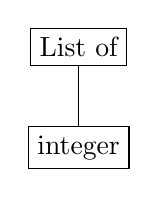
\begin{tikzpicture}
		\node[align=center, draw] (root)
		  {List of}
		;
		
    \draw (root) -- +(0, -1) node[draw, anchor=north](q) {integer};
		%  +(0,-1) 
\end{tikzpicture}
\end{center}
\begin{center}
\textbf{(C) List of Temperatures}
\end{center}
\end{minipage}
\vspace{1cm}
\tikzset{
    bnode/.style = {   
        align=center, draw,
        rectangle split, rectangle split horizontal,
				rectangle split draw splits=false, rectangle split parts=4
    }
}
\begin{tikzpicture}
		\node[bnode]
       (root)
       {	\nodepart{one}
					Dictionary of:
					\nodepart{two}
          ``blacksburg'' ,
					\nodepart{three}
					``newark'',
					\nodepart{four}
					``venice''
					};
		
    \draw (root.two south) -- +(0, -1) node[draw, anchor=north](q) {integer};
    \draw (root.three south) -- +(0, -1) node[draw, anchor=north](q) {integer};
		\draw (root.four south) -- +(0, -1) node[draw, anchor=north](q) {integer};
		%  +(0,-1) 
\end{tikzpicture}

\begin{center}
\textbf{(B) Dictionary of Weathers}
\end{center}

\end{center}
\caption{The same dataset can be structured differently according to the lesson at hand}
\label{data-maps-weather}
\end{figure}
    
    
\begin{figure}
    \begin{center}
    	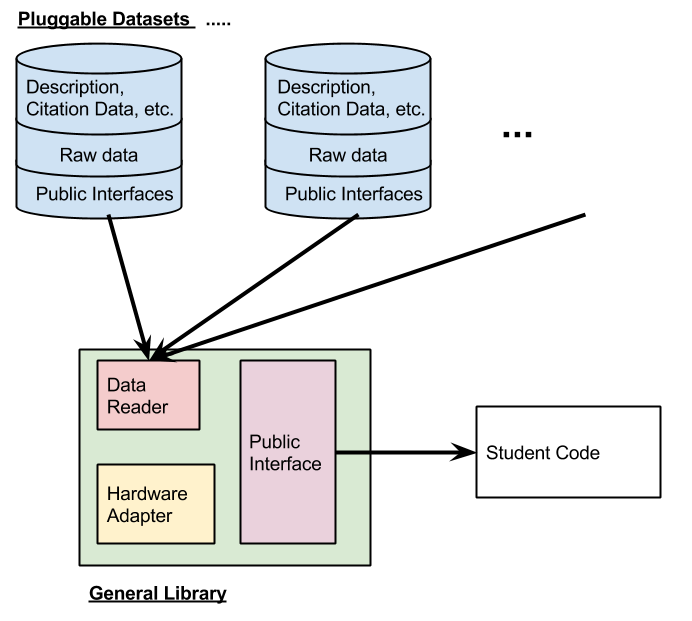
\includegraphics[width=.5\linewidth]{images/corgisDatasetArchitecture.png}
    \end{center}
    \caption{The proposed CORGIS Dataset Library Structure}
    \label{fig-corgis-architecture}
\end{figure}
    
    \textbf{RQ 1.2 Solution: An evolution of the RTW Online Building tool to make it even easier to prepare a JSON/CSV data source into a library.}
    
    This new version of the Online Building Tool will have features to reshape and organize a dataset, including ways to create data caches and artificial reworkings of the dataset according to instructor-supplied constraints.
    Specifically, the tool will be able to work with several different data formats, including CSV, JSON, SQL, and TXT, and be able to write definitions to connect to online APIs.
    Instructors will be able to write commands and queries to transform the data according to certain common functions or by using a regular query syntax.
    Figure \ref{data-maps-weather} demonstrates how the same dataset can be parred down into different structures.
    Specifically,  the tool will be able to manipulate datasets to have a desired shapes by restructuring the data according to certain common templates and high-level instructions given by the instructor.
    For example, consider a dataset of car makes and models over years with the columns ("year", "make", "model", "company"); this dataset could be grouped by year in order to make it easier for students to create bar charts in matplotlib (which would otherwise require the student to write grouping code).
    The other crucial new feature of the builder will be the ability to specify constraints and rules to generate artificial data for testing or to expand a data source, such as fake weather reports for the weather library.
    This use of mocking is a powerful way to provide more controlled learning experiences for learners.
    The output of the tool will be pluggable datasets suitable for the CORGIS architecture, rather than specific language bindings.
    
    \subsubsection{RQ 1.3: CORGIS Gallery}
    
    \textbf{How can we support students' and instructors discovery of their data source?}
    
	Instructors have a choice to assign students a specific library, a choice of libraries, or to give students freedom to choose their own library.
    There are motivational and pedagogical trade-offs to consider, but this decision lies with the instructor.
    The goal of the CORGIS library is to allow the instructors to be as flexible as they want in assigning a dataset.
    
    Currently, the list of CORGIS libraries is represented as a flat list of the libraries' names in a wiki structure \footnote{\url{http://think.cs.vt.edu/wiki/index.php/Category:Library}}. Each library has an ad-hoc page of information which may or may not include code examples, library description, and a link to the source code. As the selection grows, this informal representation becomes more and more inadequate for finding a suitable library and learning more about its nature. Originally, the gallery was a dynamically generated page based on a separate specification of the libraries (separate from the libraries themselves) -- this was too difficult to keep in sync with the libraries as they changed. The Wiki technology was adopted to make it simpler to make quick updates, but that just exacerbated the problem of keeping the library documentation up-to-date.
    
    \textbf{RQ 1.3 Solution: An enhancement to the RTW Online Gallery to make it more interactive and guiding for students to discover their datasets}
    
    I propose to make a new version of the RTW Gallery for the CORGIS project with three design goals:
    \begin{enumerate}
    \item Support instructors and students finding a suitable dataset. Provide features for both browsing and searching for libraries, especially for students who might have limited domain knowledge.
    \item Support students looking up information about a library. Provide accessible information about the origin of the data source, the abstractions that it uses, citation data, information about the data's structure and fields, the interface exposed to access the data, any important limitations and features of the dataset, and other metadata relevant to the learner.
    \item Keep the publicly available information of a dataset in sync with the datasets source. In particular, make it easy for developers to update the dataset or the metadata for the dataset, without requiring interaction with the server.
    \end{enumerate}
    
    In the case of the first two design goals, success will be measured qualitatively through the motivation and usability interviews described in section 7.2.
        
\subsection{Research Question 2: Impact}

\textbf{How do the student-driven data context and scaffolds impact students' motivation and engagement?}

	In this proposal, I seek to study how the context and facilitations affect students self-reported motivation and the more quantifiable outcomes of engagement.
    The data to answer these questions will be collected over the course of a semester in an undergraduate Computational Thinking course. Students will be surveyed twice (pre-/post-) and interviewed individually about their experiences. Performance data will be collected in the course.
    
    \subsubsection{RQ 2.1: Motivation}
    
    \textbf{What is the impact on motivation?}
    
    As previously described, the MUSIC Model states that Motivation comes through five different avenues: sense of empowerment (agency), sense of usefulness, sense of success (self-efficacy), interest, and a sense of being cared for.
    I seek to understand how a students' motivation to engage in the course changes over the semester, particularly in relation to the content, context, and scaffolds of the course. 
    
    \textbf{RQ 2.1 Solution: Measured through self-reported quantitative surveys and qualitative interviews}
        
    The MUSIC model has an associated instrument named the Music Model of Academic Motivation Instrument (MMAMI) that can be used to quantitatively measure these attributes, but MMAMI will not be used in this study; the instrument is 26 questions long and is more targeted towards formative, holistic course revision than measuring the motivation attributable to course components.
    For instance, the instrument queries students about ``the coursework'', and making the survey more specific extends the length too far.
    Instead, a custom survey based directly on the MUSIC model will be used to collect quantitative data about the students' motivation.
    This survey is given at the start of the semester (using the future-tense) and the end of the semester (using the past-tense).
    
    The complete text of this survey is included in Appendix A. However, to summarize the survey, there are two main parts.
    The first half is five series of five 7-point likert statements (Strongly Disagree -> Strongly Agree). Each series relates to a different part of the MUSIC model (``I believe it will be interesting to...''), and each likert statement relates to a different part of the course:
    \begin{itemize}
    \item "... learn to write computer programs" - course content related to algorithms.
    \item "... learn to work with abstraction" - course content related to abstraction.
    \item "... learn about the social impacts of computing" - course content related to social ethics.
    \item "... work with real-world data related to my major" - course context related to data science.
    \item "... work with my cohort" - course scaffold related to the collaborative nature of the course.
    \end{itemize}
    
    These five elements were chosen as some of the most clear and important elements of the course that would be visible and understandable to a student at both the beginning and ending of the course.
    Although there are other course elements that would be desirable to gather data on (e.g., the block-based environment), there is a limited number of questions that we can ask students. 
    These questions should be considered formative, as new elements might be added in future semesters.
    For now, these questions get at the three main course content objectives, the course context, and one of the most visible scaffolds available to students.
    
    The second half of the survey instrument has five open-ended qualitative questions relating to the components of the MUSIC model, phrased to ask for particularly extreme examples of motivating and demotivating aspects: for example, the first question is ``So far, what parts of the course seem particularly interesting or boring to you?''. While the first half of the survey will give structured data about the components of the course, this section will give rough data about the ``stand-out'' parts. The data collected will be analyzed using a grounded method to establish recurring themes in the course components -- for instance, a large percentage of students might report that the block-based environment made them feel particularly successful.
    
    The data gathered using this instrument will be used to answer the following specific subquestions:
    
    \begin{enumerate}
    \item What are students initial, self-reported attitudes and expectations entering the course?
    \item How does students' motivation change over the course of the semester?
    \item What course components are particularly effective or not effective at providing motivation?
    \item Do different course components affect different aspects of motivation in different ways (e.g., scaffolds would be expected to affect success, but do they also have an impact on sense of usefulness or interest?)
    \end{enumerate}
    
	In addition to the survey, a sample of students will be interviewed near the end of the semester in order to gather rich qualitative data specifically on the use of the data science context (as opposed to the course components in general).
    I will attempt to select students to gather a representative distribution of the population as a whole, but this will be limited by the volunteer nature of the interviews.
    Questions will be asked relating to the students motivation towards the dataset, but also about the usability of their experience.
    The interview will be conducted over a period of roughly 30-45 minutes and will be audio recorded to make analysis easier.
    
    The complete protocol for the interview is given in Appendix B. The interview will begin an introduction describing the overal goal, and some questions about the current status of the student. Then they will be questioned on their dataset in general and in relation to the five components of the music model (e.g., ``What aspects of your dataset did you have control over?''). Finally, they will be asked an open-ended question about the dataset.
    
    The data collected in the survey will be used to answer the following subquestions:
    
    \begin{itemize}
    \item What aspects of the dataset experience affected the students' motivation?
    \item Do the students understand how to use the dataset?
    \item Do students generally expect the dataset to be authentic and relate to the real-world?
    \item How do students view the data science context in comparison to the rest of the course?
    \end{itemize}
                
    \subsubsection{RQ 2.2: Engagement}
    
    \textbf{What is the impact on engagement?}
    
    Within this proposal, I define engagement as the outcomes of motivation, as opposed to motivation itself which is internal and non-observable.
    There are a wide range of outcomes that can be classified as potential outcomes of engagement. 
    These outcomes represent desirable behavior from students that should be affected by their internal motivation.
    I will analyze students engagement in order to find what can be predicted by their motivation.

    \textbf{RQ 2.1 Solution: Measured through observable outcomes and some self-reported information}
    
    In order to do this analysis, I will collect several different outcomes of their observed behavior.
    The following is a list of the outcomes I will be measuring, and their source:
    
    \begin{description}
    \item[Attendance] Measured as a numeric value indicating how many classes they attended. This is a normal part of the course metrics, since attendance influences a students' grade.
	\item[Procrastination] Measured as a number indicating how many times the student handed in an assignment late.
    \item[Assistant Observations] Measured as two numbers that reflect the students' primary teaching assistant assessment of the students' motivation and ability. This will be collected near the end of the semester.
    \item[Course Performance] Measured as several numbers based on the students' performance in each of the different phases of the course.
    \item[Project Performance] Measured as a cumulative number based on the students' performance on the final data science project (which is evaluated according to a rubric by multiple reviewers within the course).
    \item[Intent to Continue] The survey includes a single engagement question, asking if students intend to continue their computing education (7-point likert, Strongly Disagree to Strongly Agree).
    \end{description}
    
    It is possible that further self-reported outcomes could be added to this list in the future.
    
    \begin{figure}
    \begin{center}
    	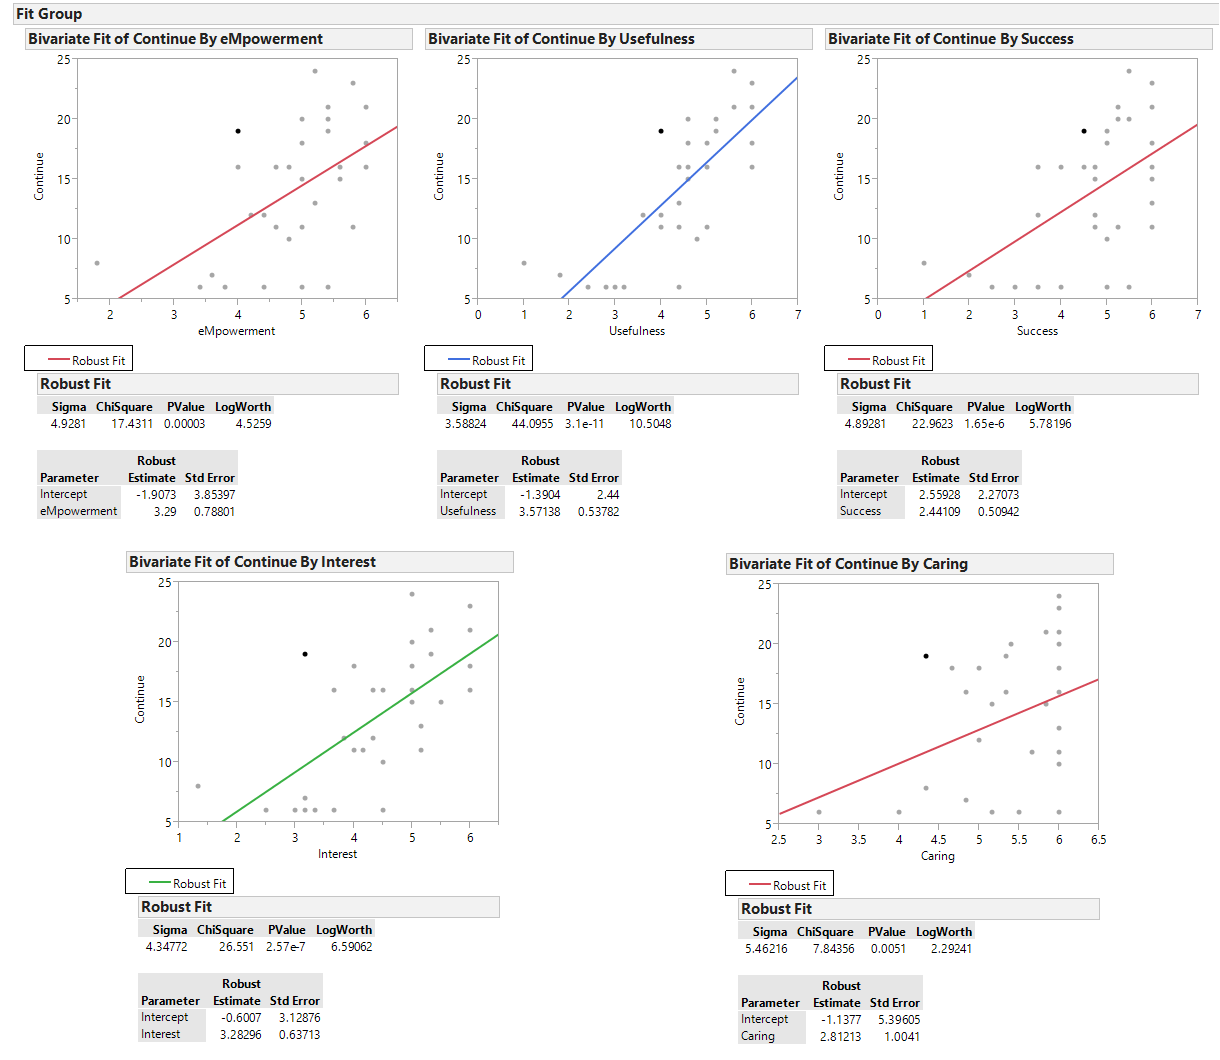
\includegraphics[width=\linewidth]{images/continue-vs-motivation.png}
    \end{center}
    \caption{Students intent to continue their computing education vs. their self-reported motivation. Usefulness might be a better predictor than Interest or Caring (N=35).}
    \label{fig-continue-motivation}
\end{figure}
    
    I will analyze the relationship of each of these outcomes with the motivation data collected in the first question. In particular, I am looking for what aspects of motivation can be used to predict engagement outcomes.
    For example, preliminary data (shown in Figure \ref{fig-continue-motivation}) gathered in prior versions of the survey suggests that students' sense of the usefulness of the material is a more accurate predictor of whether they intend to continue in computing than their interest in the material (N=35).
    The data collected in that figure comes from a survey more strongly based off MMAMI, which means that it only asks about motivation at the course level, not at the course component level.
    With the new survey instrument, I hope to find out whether student's motivation towards some course elements are better predictors of the engagement outcomes than others.
    I also expect to see improvements in students' engagement outcomes related to the data science project as the technology backing the project (proposed in the previous subsection) is improved from semester to semester.

\section{Work and Publication Plan}

This section outlines a schedule for my research over the next two years, starting from this fall.

\begin{easylist}[itemize]
& Fall 2015
&& SIGCSE'16 Paper describing Python CORGIS integration into BlockPy, the block-based programming environment used int he course (submitted)
&& Third offering of CT course, collect data (N=35)
&& First version of new CORGIS Architecture
& Spring 2016
&& Fourth offering of CT course, collect data (N=30-60?)
&& First version of the new CORGIS Gallery
& Summer 2016
&& First version of the new CORGIS Builder
& Fall 2016
&& Finalization of all major CORGIS architectures
&& Fifth offering of CT course, collect data (N= expected 80?)
&& SIGCSE'17 Paper on the CORGIS project
& Spring 2017
&& Sixth offering of CT course, collect data (N=80?)
&& TOCE Journal Paper as a summative view of my primary research questions (using CORGIS to meaningfully motivate and guide large quantities of students to success).
&& Final Thesis Defense
\end{easylist}
\section{Conclusion}

My research is focused on motivating introductory computer science classes with broadly applicable contexts.
I seek to introduce new tools and approaches that can support instructors, developers, and learners in using data science and datasets as an introductory context.
In this preliminary proposal, I describe the technical work and how it will be deployed and evaluated in real classroom settings.
I anticipate that this approach to introductory computing will provide useful new techniques and tools instructors.
The research results that I uncover will advance the literature.
Thank you for taking the time to read through it!
% chapter 1: introduction
%\input{include/sections/1_introduction/introduction.tex}

% chapter 2: related work
%\input{include/sections/2_relatedwork/relatedwork.tex}

% chapter 3: system frontend walkthrough and use cases 
%\input{include/sections/3_system_frontend/system_frontend.tex}

% chapter 4: the system itself
%\input{include/sections/4_system_backend/system_backend.tex}

% chapter 5: system evaluation
%\input{include/sections/5_evaluation/evaluation.tex}

% chapter 6: conclusions
%\input{include/sections/6_conclusions/conclusions.tex}

% reference
\bibliographystyle{abbrv}
\bibliography{references}

\begin{appendices}

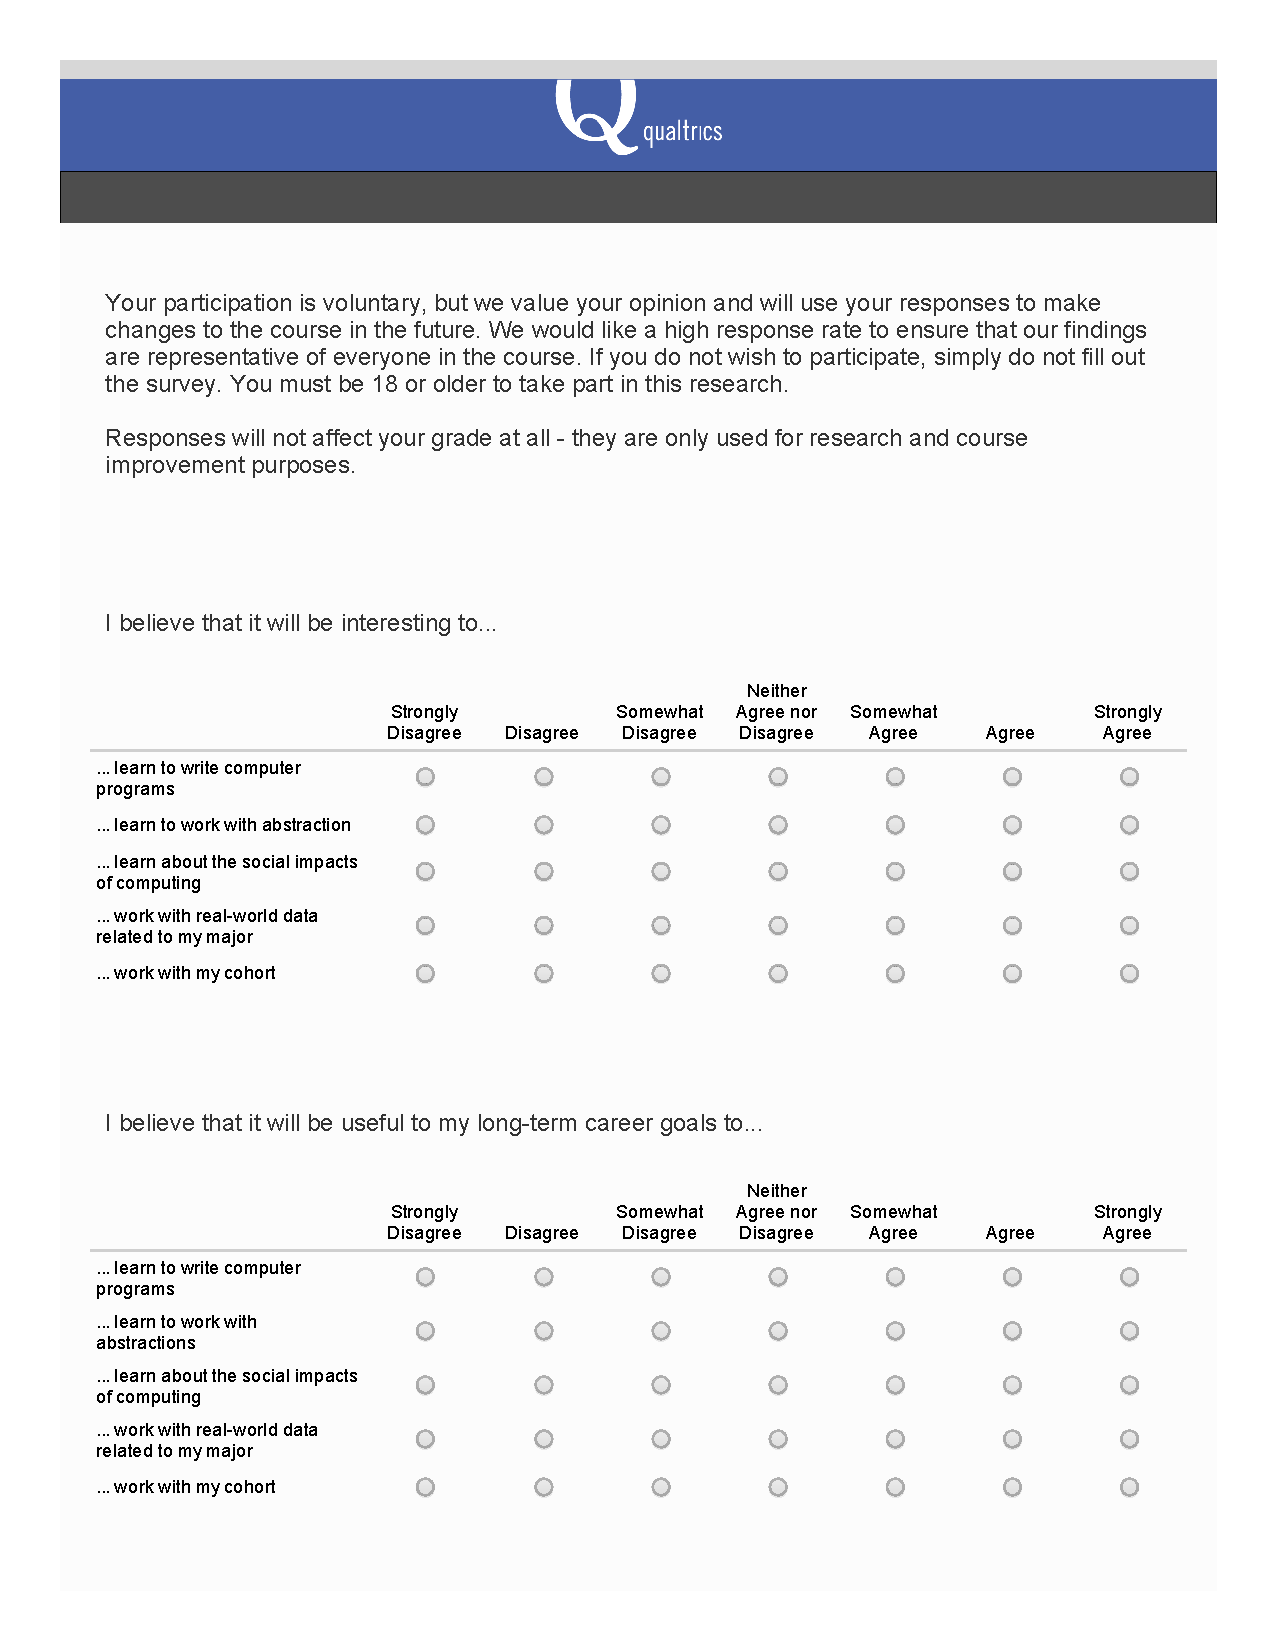
\includepdf[pages=1, scale=0.7, pagecommand=\section{Motivation Survey (Pre)}]{pdfs/ct-survey-first.pdf}
\includepdf[pages=2-, scale=0.7, pagecommand={}]{pdfs/ct-survey-first.pdf}

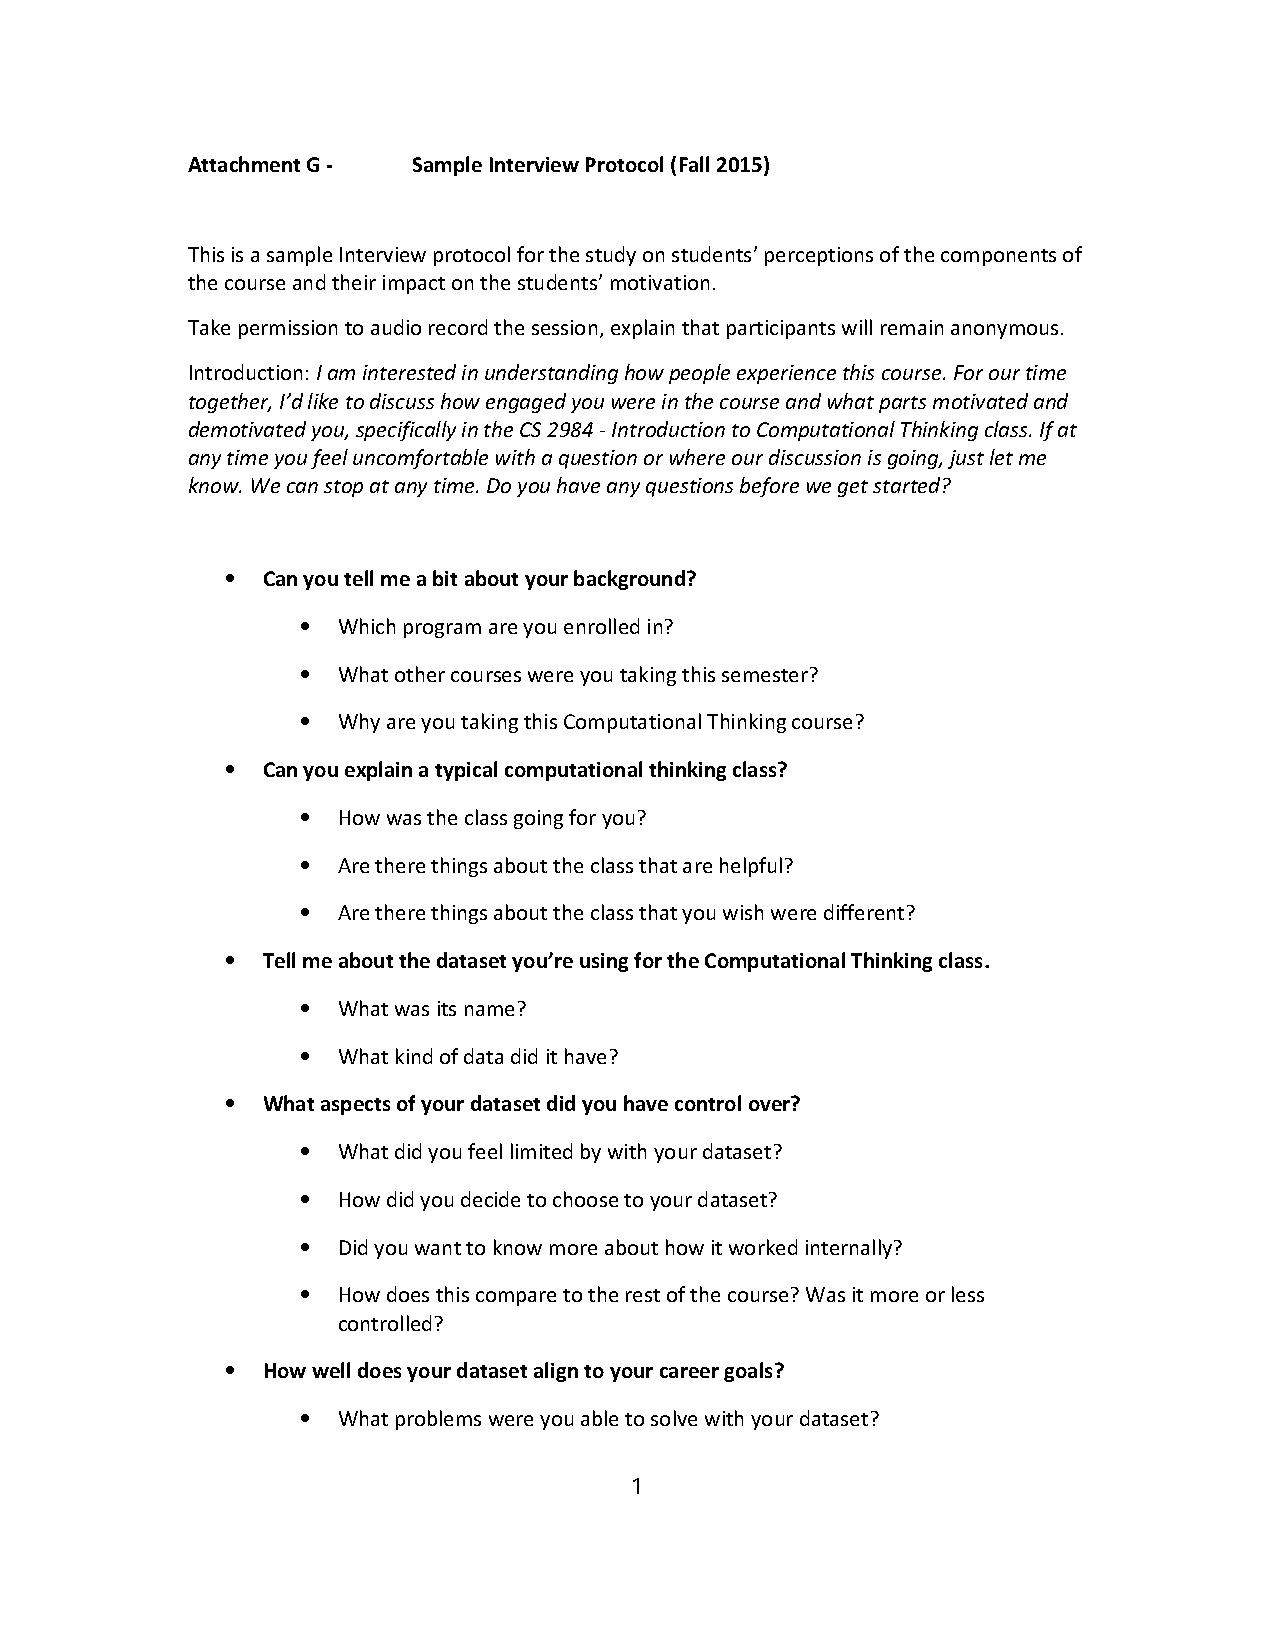
\includepdf[pages=1, scale=0.7, pagecommand=\section{Motivation Interview}]{pdfs/ct-interview.pdf}
\includepdf[pages=2-, scale=0.7, pagecommand={}]{pdfs/ct-interview.pdf}
%  \input{include/sections/A_survey/survey.tex}
  %\input{include/sections/B_open_ended_responses/open_ended_responses.tex}
\end{appendices}


\end{document}
